%\documentclass [spanish,a4paper,twoside,openany]{book}
\documentclass[english,a4paper,twoside]{article}
\usepackage{lmodern}
\usepackage[utf8]{inputenc}
\usepackage[T1]{fontenc}
\usepackage[english]{babel}
%\spanishdecimal{.}
\usepackage{epsfig}
\usepackage{amsmath}
\usepackage{alltt}
\usepackage{geometry}
\usepackage[T1]{fontenc}
\usepackage[utf8]{inputenc}
\usepackage{lastpage}
\usepackage{fancyhdr}
\usepackage{longtable}
\usepackage{titlesec}
\usepackage{aeguill}
%%\usepackage{minitoc}
\usepackage{shadow}
\usepackage{calc}
\usepackage{ifthen}
\usepackage{textcomp}
\usepackage{multirow}
\usepackage{wasysym}
\usepackage{gensymb}
\usepackage{textcomp}
\usepackage{supertabular}
\usepackage{import}
\usepackage{graphicx}
\usepackage{marvosym}
\usepackage{url}
\usepackage{hyperref}
\usepackage[table]{xcolor}
\usepackage{pdfpages}

%%Geometría de la página.


\pagestyle{fancy}
\fancypagestyle{plain}{
\fancyhf{} %anula los valores de fancy por defecto 

\fancyfoot[LE]{page \thepage\ of \pageref{LastPage}}
%\fancyfoot[CE]{\includegraphics[height=4.5mm]{anagrama/anagrama_XC_memorias}}
\fancyfoot[RE]{\emph{rev. \revision}}

\fancyfoot[LO]{\emph{\date}}
%\fancyfoot[CO]{\includegraphics[height=4.5mm]{anagrama/anagrama_XC_memorias}}
\fancyfoot[RO]{page \thepage\ of \pageref{LastPage}}
\renewcommand{\headrulewidth}{0pt} %Dibuja una raya debajo de la cabecera
\renewcommand{\footrulewidth}{0pt}
}

\renewcommand{\headrulewidth}{0.1pt} %Dibuja una raya debajo de la cabecera
\renewcommand{\footrulewidth}{0pt}
\geometry{a4paper}
\textheight= 22cm %%Espacio vertical para el texto.
%\textwidth=16cm
\marginparwidth=0mm

\fancyhf{} %anula los valores de fancy por defecto 

\fancyhead[LE]{\textsc{\titdocum}}
%\fancyhead[RO]{\textsc{\leftmark}}
\fancyhead[RO]{\textsc{\rightmark}}

\fancyfoot[LE]{page \thepage\ of \pageref{LastPage}}
%\fancyfoot[CE]{\includegraphics[height=4.5mm]{anagrama/anagrama_XC_memorias}}
\fancyfoot[RE]{\emph{rev. \revision}}

\fancyfoot[LO]{\emph{\date}}
%\fancyfoot[CO]{\includegraphics[height=4.5mm]{anagrama/anagrama_XC_memorias}}
\fancyfoot[RO]{page \thepage\ of \pageref{LastPage}}



\usepackage{array, boldline, makecell, booktabs}
\newcommand\btrule[1]{\specialrule{#1}{0pt}{0pt}}
\usepackage{colortbl}
\usepackage{multicol,caption}               % three-column layout
%\usepackage[font={footnotesize}]{caption}
\usepackage{xcolor}
\usepackage{hyperref}
\newenvironment{Figure}
  {\par\medskip\noindent\minipage{\linewidth}}
  {\endminipage\par\medskip}
\usepackage{caption}
\usepackage[section]{placeins}
%\maxdeadcycles=300

\title{Foundation Calculation Report: «1750 OX Residences - 1750 N Oxford Ave. - Eau Claire, WI» }
\author{XC structural engineering}
\date{\today}
\newcommand{\revision}{0.0}
\newcommand{\titdocum}{Foundation Calculation Report}
\begin{document}
\maketitle
\tableofcontents
\listoftables
\listoffigures
\section{Introduction and scope}
This report describes the calculation procedure and data considered in order to design the structure of a new apartment building in Eau Claire, Wisconsin.

The construction consists in a three-story apartment building with a first-floor footprint of about 19,500 square feet, a below-grade parking garage with a footprint of about 27,200 square feet, perimeter retaining walls, a slab-on-grade, and a conventional foundation system.

The first floor system is precast hollow core concrete plank on precast beams and columns. For the upper floors and roof, the system is wood-framed. Retaining walls and slab on grade are comprised of cast in place concrete, except for three reinforced CMU walls next to the garage aisles, that will be demolished during the second phase of construction.

The foundation uses conventional cast in place concrete footings to transfer axial compression and lateral loads to the ground.



\section{Building codes}
The following building and material codes were used for the design:
\begin{itemize}
\item {Building code}
  \begin{itemize}
  \item International Building Code, 2018 Edition (IBC 2018) with reference to Minimum Design Loads for Buildings and Other Structures by the American Society of Civil Engineers, 2016 Edition (ASCE 7).
    \end{itemize}
\item {Material codes}
  \begin{itemize}
  \item Reinforced Concrete: Building Code Requirements for Structural Concrete and Commentary by the American Concrete Institute, 2019 Edition (ACI 318).
    \item Masonry: Building Code Requirements and Specification for Masonry Structures and Companion Commentaries, 2013 Edition (ACI 530/530).
    \end{itemize}
\end{itemize}  

\section{Loading criteria}
A summary of the project-specific loading criteria follows (see appendix A for a detailed list of load values).

\subsection{Gravity loading}
The gravity loads listed in Table \ref{grav_load} are in addition to the self weight of the structure. The minimum loading requirements were taken from ASCE 7 as well as the loading criteria supplied by the engineer of record. Loads are given in pounds per square foot (psf).

\begin{table}[h]
  \begin{center}
   \caption{\textbf{Gravity Loads}} \label{grav_load}
   \begin{tabular}{lll}
      \textbf{Use} & \textbf{Live Loading} & \textbf{Superimposed} \\
      &&\textbf{Dead Loading} \\
      \hlineB{2}
      Parking Garage & 40 & 3 \\
      \arrayrulecolor{gray}\hline
      Storage/HVAC & 125 & 28 \\
      \arrayrulecolor{gray}\hline
      Stairways, exits & 100 & 28 \\
      \arrayrulecolor{gray}\hline
      Level 1 residential & 40 & 28 \\
      \arrayrulecolor{gray}\hline
      Level 1 corridors & 100 & 28 \\
      \arrayrulecolor{gray}\hline
      Level 1 office, recreational & 100 & 28 \\
      \arrayrulecolor{gray}\hline
      Level 1 courtyard (footprint) & 150 & 150 \\
      \arrayrulecolor{gray}\hline
      Elevated levels residential & 40 & 28 \\
      \arrayrulecolor{gray}\hline
      Elevated levels corridors & 40 & 28 \\
      \arrayrulecolor{gray}\hline
      Cornices & 60 & - \\
      \arrayrulecolor{gray}\hline
      Balconies & 40 & 28 \\
      \arrayrulecolor{gray}\hline
      Roof & 20 & 28 \\
      \hlineB{2}
  \end{tabular}
  \end{center}
\end{table}

In addition to these uniform slab loads, a perimeter dead load of 12 psf was applied to the structure to account for the weight of the cladding system.

\subsection{Wind design criteria}
Wind loading is in accordance with the IBC and ASCE 7 requirements as shown in Table \ref{wind_load}.
\begin{table}[h]
  \begin{center}
  \caption{\textbf{Wind Design Criteria}} \label{wind_load}
    \begin{tabular}{ll}
      \textbf{Parameter} & \textbf{Value} \\
      \hlineB{2}
Basic Wind Speed, 3-second gust (ultimate) & 115 mph \\
      \arrayrulecolor{gray}\hline
Basic Wind Speed, 3-second gust (nominal) & 90 mph \\
      \arrayrulecolor{gray}\hline
Exposure & B \\
      \arrayrulecolor{gray}\hline
Occupancy Category & II \\
      \arrayrulecolor{gray}\hline
Importance Factor ($I_w$ ) & 1.0 \\
      \arrayrulecolor{gray}\hline
Topographic Factor ($K_{zt}$ ) & 1.0\\
      \arrayrulecolor{gray}\hline
Enclosure Classification & Enclosed \\
      \arrayrulecolor{gray}\hline
Mean Roof Height (h) & 33' \\
      \hlineB{2}
  \end{tabular}
  \end{center}
\end{table}

\subsection{Snow loading}
Wind loading is in accordance with the ASCE 7 requirements as shown in Table \ref{snow_load}.
\begin{table}[h]
  \begin{center}
  \caption{\textbf{Snow Design Criteria}} \label{snow_load}
    \begin{tabular}{ll}
      \textbf{Parameter} & \textbf{Value} \\
      \hlineB{2}
Ground snow load $p_g$ & 60 psf \\ 
      \arrayrulecolor{gray}\hline
Terrain category & B \\
      \arrayrulecolor{gray}\hline
Exposure factor $C_e$ &  1.0 \\
      \arrayrulecolor{gray}\hline
Thermal factor $C_t$ & 1.0 \\
      \arrayrulecolor{gray}\hline
Occupancy Category & II \\
      \arrayrulecolor{gray}\hline
Snow load importance factor $I_s$ & 1.0\\
      \arrayrulecolor{gray}\hline
Snow load flat roof & 42 psf \\ 
      \hlineB{2}
  \end{tabular}
  \end{center}
\end{table}

\section{Seismic design criteria}
Seismic loads are in accordance with the IBC requirements as shown in Table \ref{seism_load}.
\begin{table}[h]
  \begin{center}
  \caption{\textbf{Seismic Design Criteria}} \label{seism_load}
    \begin{tabular}{ll}
      \textbf{Parameter} & \textbf{Value} \\
      \hlineB{2}
Building Latitude/Longitude & 44$^o$49'01.8"N 91$^o$30'34.8"W \\
      \arrayrulecolor{gray}\hline
Occupancy Category & II\\
      \arrayrulecolor{gray}\hline
Importance Factor $I_e$ &  1.0\\
      \arrayrulecolor{gray}\hline
Mapped Spectral Acceleration & $S_s$ = 0.045; $S_1$ = 0.038 \\
      \arrayrulecolor{gray}\hline
Site Class & B \\
      \arrayrulecolor{gray}\hline
Site Class Coefficients & $F_a$ = 1.0; $F_v$ = 1.0 \\
      \arrayrulecolor{gray}\hline
Spectral Response Coefficients & $S_{DS}$ = 0.03; $S_{D1}$ = 0.025 \\
      \arrayrulecolor{gray}\hline
Seismic Design Category & A \\
      \hlineB{2}
  \end{tabular}
  \end{center}
\end{table}



\section{Materials}
The material properties used for the design are summarized in Tables \ref{conc_mat} and \ref{reinf_mat}.
\begin{table}[h]
  \begin{center}
   \caption{\textbf{Concrete properties}} \label{conc_mat}
  \begin{tabular}{ll}
      \textbf{Member} & \textbf{Nominal f'$_c$} \\
      \hlineB{2}
      Footings & 3.0 ksi \\
      \arrayrulecolor{gray}\hline
      Basement Walls & 4.0 ksi \\
      \arrayrulecolor{gray}\hline
      Foundation frost walls & 4.0 ksi \\
      \arrayrulecolor{gray}\hline
      Stair landings and treads & 4.0 ksi \\
      \arrayrulecolor{gray}\hline
      Slab on grade &  4.0 ksi \\
      \hlineB{2}
  \end{tabular}
  \end{center}
\end{table}

\begin{table}[h]
  \begin{center}
   \caption{\textbf{Reinforcement properties}} \label{reinf_mat}
  \begin{tabular}{ll}
      \textbf{Standard} & \textbf{Nominal f$_y$} \\
      \hlineB{2}
      All ASTM A615 Grade 60 & 60 ksi \\
       \hlineB{2}
  \end{tabular}
  \end{center}
\end{table}
     

\section{Design and analysis software}
The computer software employed for the analysis of the structure is the Finite Element Program called \textbf{XC} (see program description at \url{http://xcengineering.xyz/html\_files/software.html}).

\section{Load combinations}
The load combinations shown in tables \ref{ULS} and \ref{SLS} follow the strength design load combinations listed in IBC, section 1605.
\begin{table}[h]
  \begin{center}
   \caption{\textbf{Combinations Ultimate Limit States}} \label{ULS}
   \begin{tabular}{lll}
    \textbf{Identifier} && \textbf{Load Combination}\\
      \hlineB{2}
    ULS01: && 1.4*D \\
      \arrayrulecolor{gray}\hline
    ULS02\_a: && 1.2*D + 1.6*Lru + Lpu + 0.5*S\\
      \arrayrulecolor{gray}\hline
    ULS02\_b: && 1.2*D + 1.6*Lrs + Lps + 0.5*S \\
      \arrayrulecolor{gray}\hline
    ULS03\_a: && 1.2*D + 1.6*S + 0.5*Lru + Lpu \\
      \arrayrulecolor{gray}\hline
    ULS03\_b: && 1.2*D + 1.6*S + 0.5*Lrs + Lps \\
      \arrayrulecolor{gray}\hline
    ULS04\_b: && 1.2*D + 1.6*S + 0.5*W\_NS \\
      \arrayrulecolor{gray}\hline
    ULS04\_a: && 1.2*D + 1.6*S + 0.5*W\_WE \\
      \arrayrulecolor{gray}\hline
    ULS05\_a: && 1.2*D + W\_WE + 0.5*Lru + Lpu \\
      \arrayrulecolor{gray}\hline
    ULS05\_b: && 1.2*D + W\_NS + 0.5*Lru + Lpu \\
      \arrayrulecolor{gray}\hline
    ULS05\_c: && 1.2*D + W\_WE + 0.5*Lrs + Lps \\
      \arrayrulecolor{gray}\hline
    ULS05\_d: && 1.2*D + W\_NS + 0.5*Lrs + Lps \\
       \arrayrulecolor{gray}\hline
    ULS06\_a: && 1.2*D + 0.5*Lru + Lpu + 0.2*S \\
      \arrayrulecolor{gray}\hline
    ULS06\_b: && 1.2*D + 0.5*Lrs + Lps + 0.2*S \\
      \arrayrulecolor{gray}\hline
    ULS07\_a: && 0.9*D + W\_WE \\
      \arrayrulecolor{gray}\hline
    ULS07\_b: && 0.9*D + W\_NS \\
    \hlineB{2}
    Where: & \multicolumn{2}{l}{} \\
    & \multicolumn{2}{l}{ D =  dead load} \\
    & \multicolumn{2}{l}{ Lru =  live load (uniform on rooms)} \\
    & \multicolumn{2}{l}{ Lrs =  live load (staggered pattern on rooms)}\\
    & \multicolumn{2}{l}{ Lpu =  live load (uniform on patios)} \\
    & \multicolumn{2}{l}{ Lps =  live load (staggered pattern on patios)}\\
    & \multicolumn{2}{l}{ S =  snow load} \\
    & \multicolumn{2}{l}{ W\_WE =  Wind West-East} \\
    & \multicolumn{2}{l}{ W\_NS =  Wind North-South} \\
  \end{tabular}
  \end{center}
\end{table}


\begin{table}[h]
  \begin{center}
   \caption{\textbf{Combinations Serviceability Limit States}} \label{SLS}
   \begin{tabular}{lll}
    \textbf{Identifier} && \textbf{Load Combination}\\
      \hlineB{2}
    SLS01: && 1.0*D \\
    SLS02\_a: && 1.0*D + 1.0*Lru + Lpu + 0.3*S \\
    SLS02\_b: && 1.0*D + 1.0*Lrs + Lps + 0.3*S \\
    SLS03\_a: && 1.0*D + 1.0*S + 0.3*Lru + 0.3*Lpu \\
    SLS03\_b: && 1.0*D + 1.0*S + 0.3*Lrs + 0.3*Lps \\
    SLS04\_a: && 1.0*D + W\_WE + 1.0*Lru + Lpu \\
    SLS04\_b: && 1.0*D + W\_NS + 1.0*Lru + Lpu \\
    SLS04\_c: && 1.0*D + W\_WE + 1.0*Lrs + Lps \\
    SLS04\_d: && 1.0*D + W\_NS + 1.0*Lrs + Lps \\
    SLS05\_a: && 1.0*D + W\_WE \\
    SLS05\_b: && 1.0*D + W\_NS \\
    \hlineB{2}
    Where: & \multicolumn{2}{l}{} \\
    & \multicolumn{2}{l}{ D =  dead load} \\
    & \multicolumn{2}{l}{ Lru =  live load (uniform on rooms)} \\
    & \multicolumn{2}{l}{ Lrs =  live load (staggered pattern on rooms)}\\
    & \multicolumn{2}{l}{ Lpu =  live load (uniform on patios)} \\
    & \multicolumn{2}{l}{ Lps =  live load (staggered pattern on patios)}\\
    & \multicolumn{2}{l}{ S =  snow load} \\
    & \multicolumn{2}{l}{ W\_WE =  Wind West-East} \\
    & \multicolumn{2}{l}{ W\_NS =  Wind North-South} \\
  \end{tabular}
  \end{center}
\end{table}

\section{Structural model}
\section{Structural model}
A three-dimensional elastic computer model of the substructure is analyzed using XC. The model includes first floor frame and columns (see figure \ref{model}). The hollow core planks ar modelled using shell elements, while beams and columns are modelled using frame elements. Loads transmited by 2$^{nd}$, 3$^{rd}$ floors and roof are applied to the 1$^{st}$. Load layout is shown in figure \ref{loadLay}. See in figures \ref{LC_D} to \ref{LC_W_NS} load distribution for each load case.\\

Linear loads are expressed in $\mathrm{kN/m}$ and surface loads in $\mathrm{kN/m^2}$, where:\\
\begin{center}
  \begin{tabular}{ll}
    1 $\mathrm{kN/m}$ = & 68.52178 lb/ft \\
    1 $\mathrm{kN/m^2}$ = & 20.885434 psf \\
  \end{tabular}
  \end{center}

\captionsetup[figure]{font=footnotesize}
\twocolumn
\begin{Figure}
    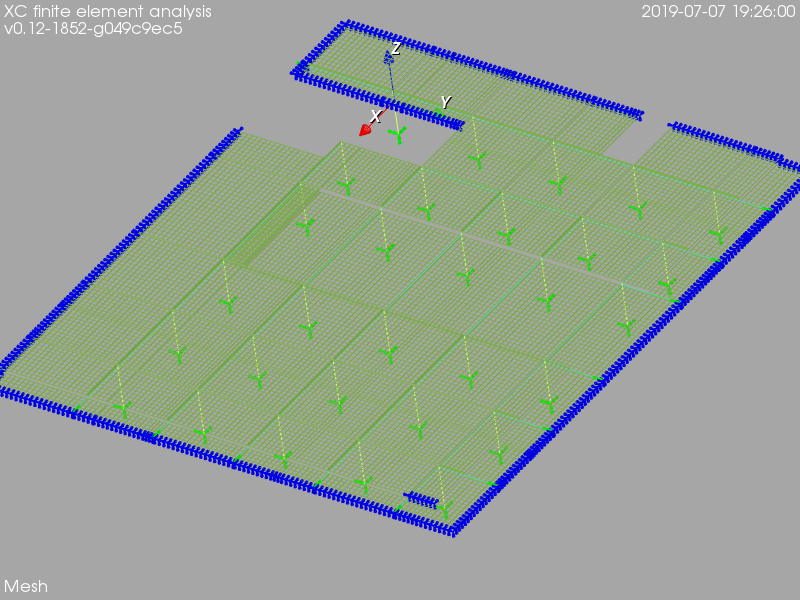
\includegraphics[width=\linewidth]{figures/mesh}
    \captionof{figure}{Elastic model, mesh.}
    \label{model}
\end{Figure}
\begin{Figure}
    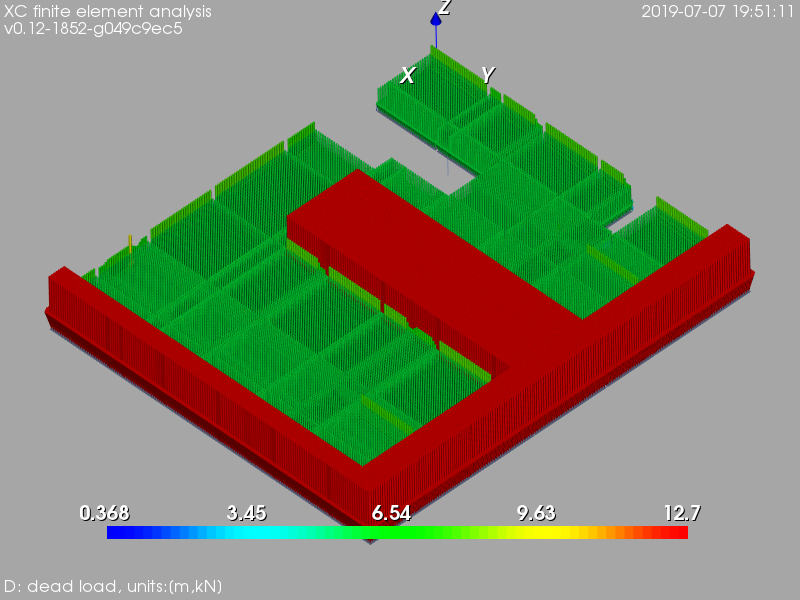
\includegraphics[width=\linewidth]{figures/LC_D}
    \captionof{figure}{Load case D: dead load (include slab selfweight) [units: kN,m].}
    \label{LC_D}
\end{Figure}

\begin{Figure}
    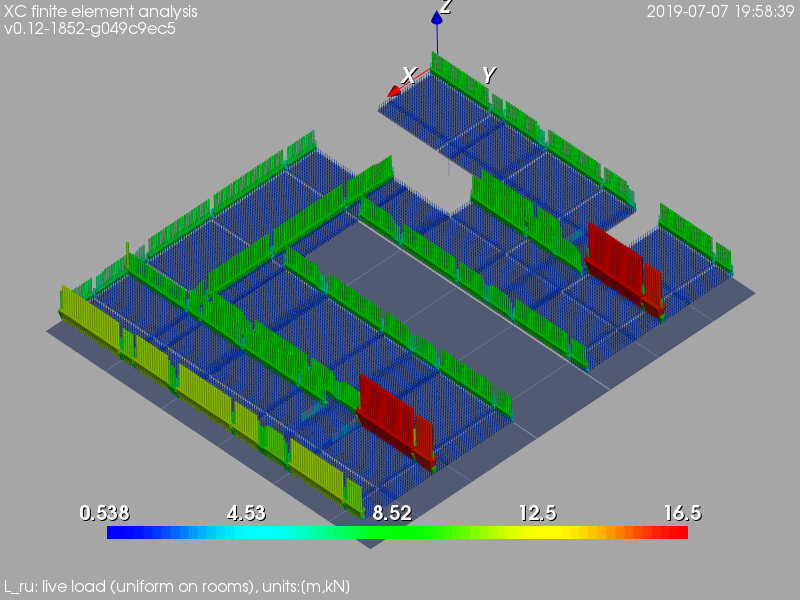
\includegraphics[width=\linewidth]{figures/LC_L_ru}
    \captionof{figure}{Load case Lru: live load (uniform on rooms) [units: kN,m].}
    \label{LC_L_ru}
\end{Figure}

\begin{Figure}
    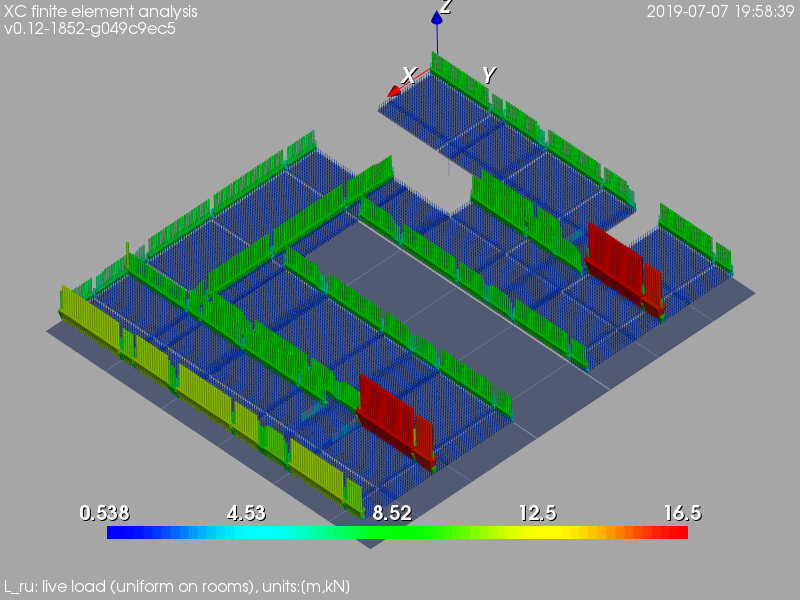
\includegraphics[width=\linewidth]{figures/LC_L_rs}
    \captionof{figure}{Load case Lrs:  live load (staggered pattern on rooms) [units: kN,m].}
    \label{LC_L_rs}
\end{Figure}

\begin{Figure}
    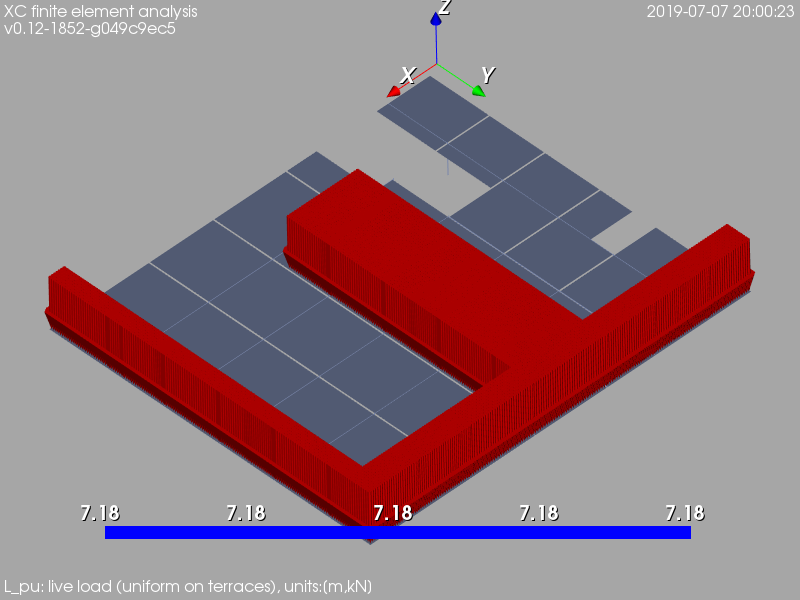
\includegraphics[width=\linewidth]{figures/LC_L_pu}
    \captionof{figure}{Load case Lpu: live load (uniform on patios) [units: kN,m].}
    \label{LC_L_pu}
\end{Figure}

\begin{Figure}
    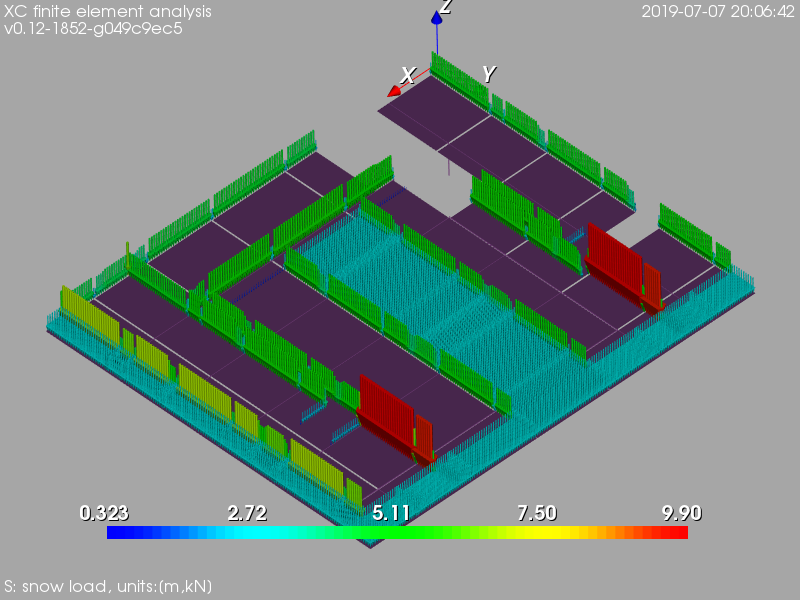
\includegraphics[width=\linewidth]{figures/LC_S}
    \captionof{figure}{Load case S: snow [units: kN,m].}
    \label{LC_S}
\end{Figure}
\begin{Figure}
    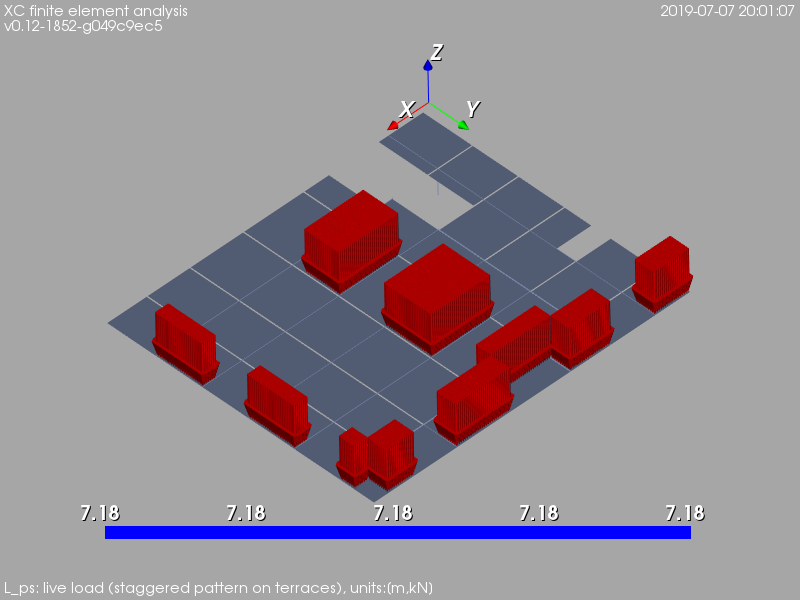
\includegraphics[width=\linewidth]{figures/LC_L_ps}
    \captionof{figure}{Load case Lps:  live load (staggered pattern on patios) [units: kN,m].}
    \label{LC_L_ps}
\end{Figure}

\begin{Figure}
    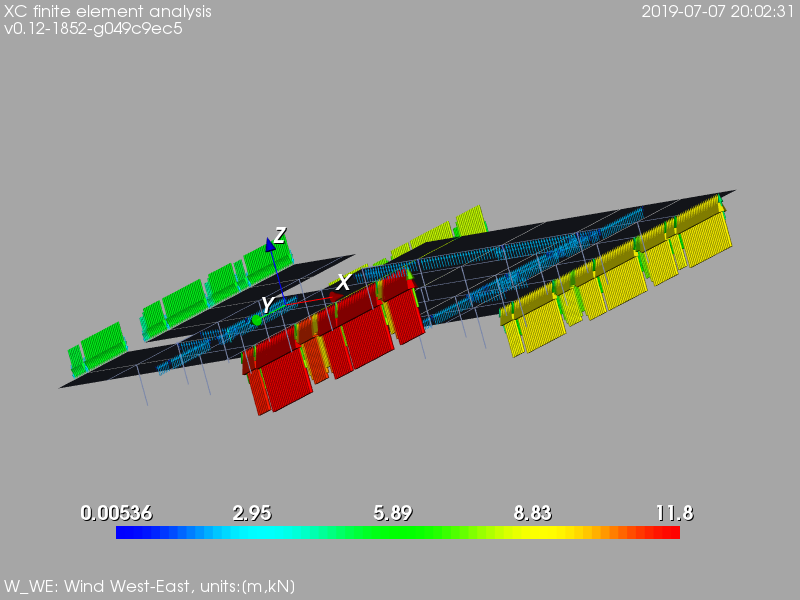
\includegraphics[width=\linewidth]{figures/LC_W_WE}
    \captionof{figure}{Load case W\_WE:  wind West-East [units: kN,m].}
    \label{LC_W_WE}
\end{Figure}

\begin{Figure}
    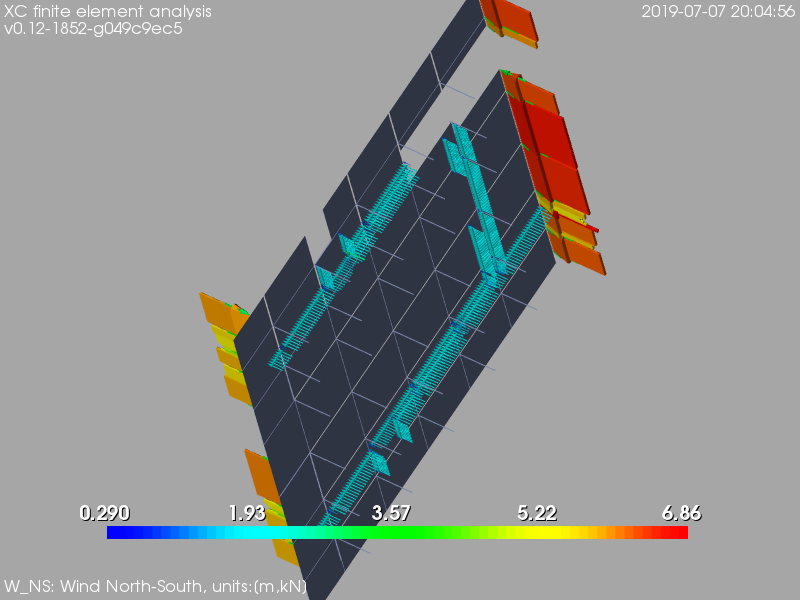
\includegraphics[width=\linewidth]{figures/LC_W_NS}
    \captionof{figure}{Load case W\_NS: wind North-South [units: kN,m].}
    \label{LC_W_NS}
\end{Figure}
\onecolumn
\begin{Figure}
    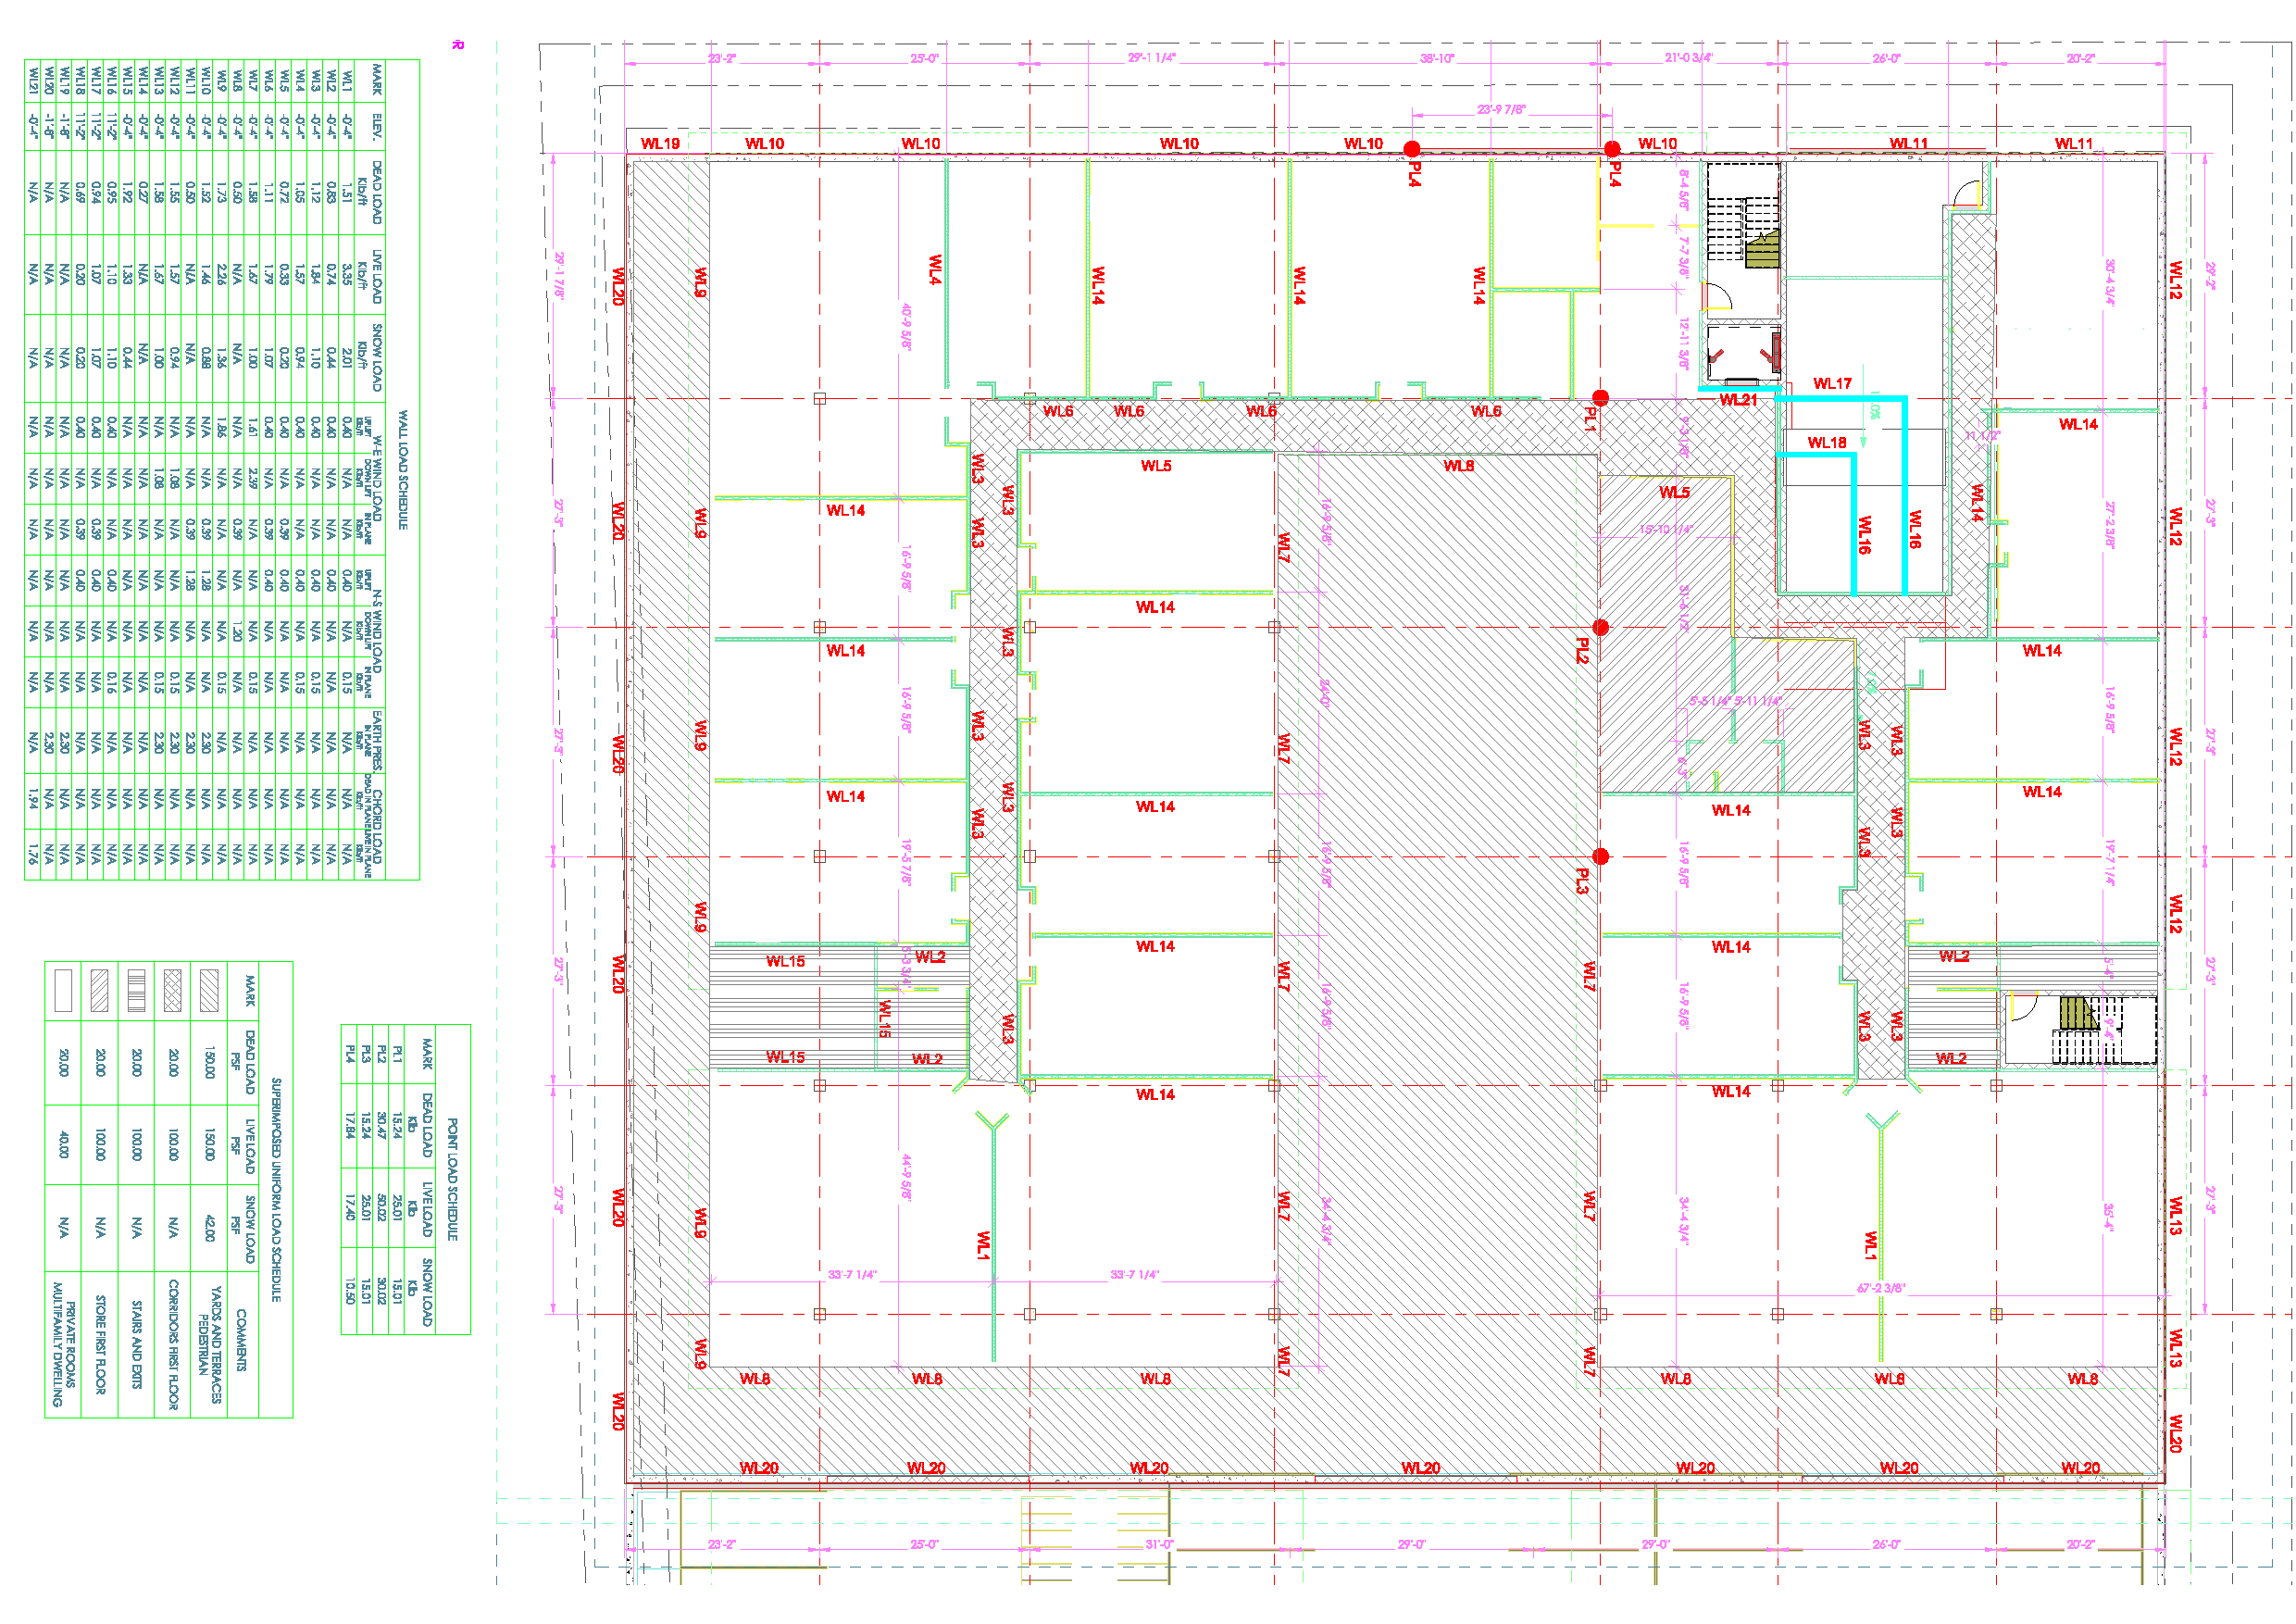
\includegraphics[width=150mm]{figures/loads_layout}
    \captionof{figure}{Load layout on first floor.}
    \label{loadLay}
\end{Figure}

\section{Footings}
\subsection{Introduction}


\subsection{Loads}
The loads acting on the footins are shown in \S \ref{sc_column_internal_forces}.

\subsection{Load combinations}
The load combinations are shown in tables \ref{ULS} and \ref{SLS}.

\subsection{Footing dimensions and reinforcement}
The dimensions and the reinforcement of the footings are indicated in the table \ref{tb_column_footing_schedule}. The position of the footing in the building grid is indicated at the last column.

\begin{table}
    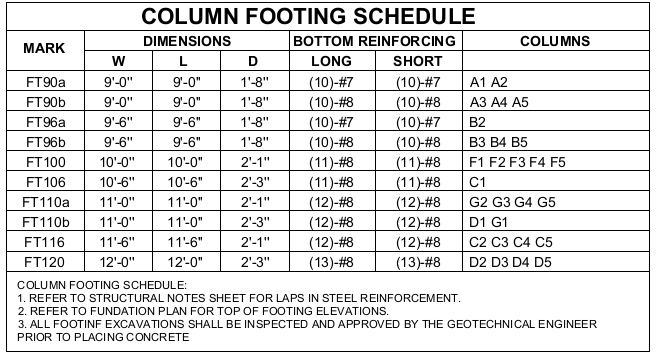
\includegraphics[width=\linewidth]{figures/column_footing_schedule.png}
    \caption{Column footing schedule.}\label{tb_column_footing_schedule}
\end{table}

\subsection{Allowable soil-bearing pressures}
The results obtained for the verification of the soil-bearing capacity are the following:

\begin{center}
  \begin{tabular}{|l|l|r|r|}
\hline
Foundation & Worst & Vertical & Capacity\\
 & combination & load (kN) & factor\\
\hline
 A1 &  SLS04\_a & -356.20 & 0.33\\
 A2 &  SLS02\_a & -644.78 & 0.60\\
 A3 &  SLS02\_a & -950.92 & 0.88\\
 A4 &  SLS02\_a & -881.82 & 0.82\\
 A5 &  SLS04\_b & -933.03 & 0.86\\
 B2 &  SLS02\_a & -670.79 & 0.56\\
 B3 &  SLS02\_a & -1,030.65 & 0.86\\
 B4 &  SLS02\_a & -968.24 & 0.80\\
 B5 &  SLS04\_b & -972.32 & 0.81\\
 C1 &  SLS02\_a & -1,460.67 & 0.99\\
 C2 &  SLS02\_a & -1,742.45 & 0.99\\
 C3 &  SLS02\_a & -1,750.31 & 0.99\\
 C4 &  SLS02\_a & -1,751.62 & 0.99\\
 C5 &  SLS02\_a & -1,660.02 & 0.94\\
 D1 &  SLS02\_a & -1,648.12 & 1.02\\
 D2 &  SLS04\_a & -1,950.01 & 1.01\\
 D3 &  SLS04\_a & -1,959.12 & 1.02\\
 D4 &  SLS04\_a & -1,960.14 & 1.02\\
 D5 &  SLS04\_a & -1,838.69 & 0.96\\
 F1 &  SLS02\_a & -1,090.88 & 0.82\\
 F2 &  SLS02\_a & -997.32 & 0.75\\
 F3 &  SLS02\_a & -1,011.87 & 0.76\\
 F4 &  SLS02\_a & -1,005.30 & 0.75\\
 F5 &  SLS04\_b & -741.90 & 0.56\\
 G1 &  SLS02\_a & -1,496.86 & 0.93\\
 G2 &  SLS02\_a & -1,256.06 & 0.78\\
 G3 &  SLS02\_a & -1,227.94 & 0.76\\
 G4 &  SLS02\_a & -1,137.75 & 0.70\\
 G5 &  SLS04\_b & -1,167.26 & 0.72\\
\hline
  \end{tabular}
  \end{center}

\subsection{Flexure design}

\begin{table}
    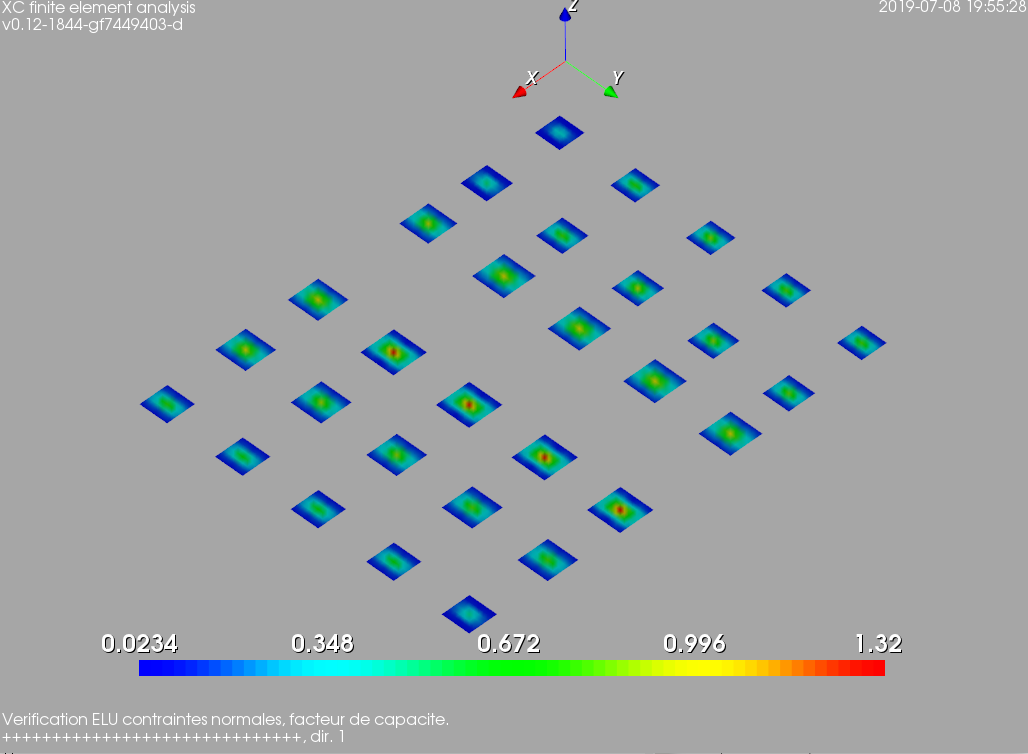
\includegraphics[width=\linewidth]{figures/flexure_design_cf_long_direction}
    \caption{Flexure in the longitudinal direction. Capacity factor.}\label{tb_flexure_design_cf_long_direction}
\end{table}

\begin{table}
    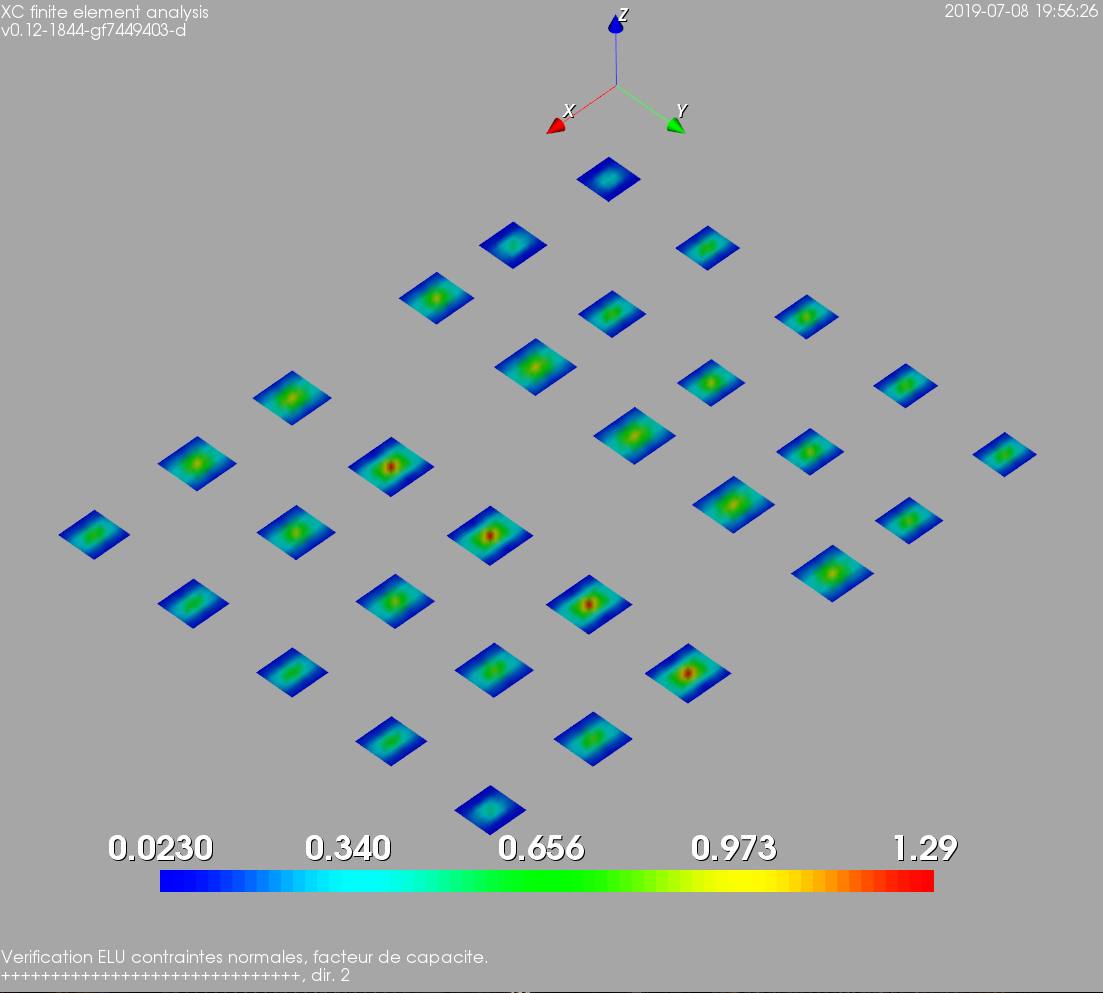
\includegraphics[width=\linewidth]{figures/flexure_design_cf_transv_direction}
    \caption{Flexure in the transverse direction. Capacity factor.}\label{tb_flexure_design_cf_transv_direction}
\end{table}

\subsection{Shear design}
The results of the shear strength verification are shown in the following table:

\begin{center}
  \begin{tabular}{|l|l|r|r|r|r|r|r|r|r|}
\hline
Footing & Worst & Vertical & thickness & l & d & c & Vd/l & Vu & CF\\
 & combination & load (kN) & (m) & (m) & (m) & (m) & kN/m & kN/m & \\
\hline
 A1 &  SLS04\_a & -356.20 & 0.51 & 2.74 & 0.46 & 0.41 & 33.66 & 280.00 & 0.12\\
 A2 &  SLS02\_a & -644.78 & 0.51 & 2.74 & 0.46 & 0.41 & 60.94 & 280.00 & 0.22\\
 A3 &  SLS02\_a & -950.92 & 0.51 & 2.74 & 0.46 & 0.41 & 89.87 & 280.00 & 0.32\\
 A4 &  SLS02\_a & -881.82 & 0.51 & 2.74 & 0.46 & 0.41 & 83.34 & 280.00 & 0.30\\
 A5 &  SLS04\_b & -933.03 & 0.51 & 2.74 & 0.46 & 0.41 & 88.18 & 280.00 & 0.31\\
 B2 &  SLS02\_a & -670.79 & 0.51 & 2.90 & 0.46 & 0.41 & 63.00 & 280.00 & 0.22\\
 B3 &  SLS02\_a & -1,030.65 & 0.51 & 2.90 & 0.46 & 0.41 & 96.79 & 280.00 & 0.35\\
 B4 &  SLS02\_a & -968.24 & 0.51 & 2.90 & 0.46 & 0.41 & 90.93 & 280.00 & 0.32\\
 B5 &  SLS04\_b & -972.32 & 0.51 & 2.90 & 0.46 & 0.41 & 91.31 & 280.00 & 0.33\\
 C1 &  SLS02\_a & -1,460.67 & 0.69 & 3.20 & 0.62 & 0.41 & 111.20 & 378.00 & 0.29\\
 C2 &  SLS02\_a & -1,742.45 & 0.64 & 3.51 & 0.57 & 0.41 & 138.68 & 350.00 & 0.40\\
 C3 &  SLS02\_a & -1,750.31 & 0.64 & 3.51 & 0.57 & 0.41 & 139.31 & 350.00 & 0.40\\
 C4 &  SLS02\_a & -1,751.62 & 0.64 & 3.51 & 0.57 & 0.41 & 139.42 & 350.00 & 0.40\\
 C5 &  SLS02\_a & -1,660.02 & 0.64 & 3.51 & 0.57 & 0.41 & 132.12 & 350.00 & 0.38\\
 D1 &  SLS02\_a & -1,648.12 & 0.69 & 3.35 & 0.62 & 0.41 & 125.50 & 378.00 & 0.33\\
 D2 &  SLS04\_a & -1,950.01 & 0.64 & 3.66 & 0.57 & 0.41 & 153.65 & 350.00 & 0.44\\
 D3 &  SLS04\_a & -1,959.12 & 0.64 & 3.66 & 0.57 & 0.41 & 154.37 & 350.00 & 0.44\\
 D4 &  SLS04\_a & -1,960.14 & 0.64 & 3.66 & 0.57 & 0.41 & 154.45 & 350.00 & 0.44\\
 D5 &  SLS04\_a & -1,838.69 & 0.64 & 3.66 & 0.57 & 0.41 & 144.88 & 350.00 & 0.41\\
 F1 &  SLS02\_a & -1,090.88 & 0.64 & 3.05 & 0.57 & 0.41 & 87.98 & 350.00 & 0.25\\
 F2 &  SLS02\_a & -997.32 & 0.64 & 3.05 & 0.57 & 0.41 & 80.44 & 350.00 & 0.23\\
 F3 &  SLS02\_a & -1,011.87 & 0.64 & 3.05 & 0.57 & 0.41 & 81.61 & 350.00 & 0.23\\
 F4 &  SLS02\_a & -1,005.30 & 0.64 & 3.05 & 0.57 & 0.41 & 81.08 & 350.00 & 0.23\\
 F5 &  SLS04\_b & -741.90 & 0.64 & 3.05 & 0.57 & 0.41 & 59.84 & 350.00 & 0.17\\
 G1 &  SLS02\_a & -1,496.86 & 0.69 & 3.35 & 0.62 & 0.41 & 113.98 & 378.00 & 0.30\\
 G2 &  SLS02\_a & -1,256.06 & 0.64 & 3.35 & 0.57 & 0.41 & 100.75 & 350.00 & 0.29\\
 G3 &  SLS02\_a & -1,227.94 & 0.64 & 3.35 & 0.57 & 0.41 & 98.50 & 350.00 & 0.28\\
 G4 &  SLS02\_a & -1,137.75 & 0.64 & 3.35 & 0.57 & 0.41 & 91.26 & 350.00 & 0.26\\
 G5 &  SLS04\_b & -1,167.26 & 0.64 & 3.35 & 0.57 & 0.41 & 93.63 & 350.00 & 0.27\\
\hline
  \end{tabular}
  \end{center}

\subsection{Two-way shear design}
The results of the punching shear strength verification are shown in the following table:

\begin{center}
  \begin{tabular}{|l|l|r|r|r|r|r|r|r|r|}
\hline
Footing & Worst & Vertical & thickness & L & d & c & Vd/l & Vu & CF\\
 & combination & load (kN) & (m) & (m) & (m) & (m) & kN/m & kN/m & \\
\hline
 A1 &  SLS04\_a & -356.20 & 0.51 & 2.74 & 0.46 & 0.41 & 92.90 & 517.97 & 0.18\\
 A2 &  SLS02\_a & -644.78 & 0.51 & 2.74 & 0.46 & 0.41 & 168.16 & 517.97 & 0.32\\
 A3 &  SLS02\_a & -950.92 & 0.51 & 2.74 & 0.46 & 0.41 & 248.00 & 517.97 & 0.48\\
 A4 &  SLS02\_a & -881.82 & 0.51 & 2.74 & 0.46 & 0.41 & 229.98 & 517.97 & 0.44\\
 A5 &  SLS04\_b & -933.03 & 0.51 & 2.74 & 0.46 & 0.41 & 243.33 & 517.97 & 0.47\\
 B1 &  SLS02\_a & -429.53 & 0.51 & 2.90 & 0.46 & 0.41 & 113.28 & 517.97 & 0.22\\
 B2 &  SLS02\_a & -670.79 & 0.51 & 2.90 & 0.46 & 0.41 & 176.91 & 517.97 & 0.34\\
 B3 &  SLS02\_a & -1,030.65 & 0.51 & 2.90 & 0.46 & 0.41 & 271.82 & 517.97 & 0.52\\
 B4 &  SLS02\_a & -968.24 & 0.51 & 2.90 & 0.46 & 0.41 & 255.36 & 517.97 & 0.49\\
 B5 &  SLS04\_b & -972.32 & 0.51 & 2.90 & 0.46 & 0.41 & 256.43 & 517.97 & 0.50\\
 C1 &  SLS02\_a & -1,460.67 & 0.69 & 3.20 & 0.62 & 0.41 & 320.25 & 699.26 & 0.46\\
 C2 &  SLS02\_a & -1,742.45 & 0.64 & 3.51 & 0.57 & 0.41 & 410.79 & 647.47 & 0.63\\
 C3 &  SLS02\_a & -1,750.31 & 0.64 & 3.51 & 0.57 & 0.41 & 412.64 & 647.47 & 0.64\\
 C4 &  SLS02\_a & -1,751.62 & 0.64 & 3.51 & 0.57 & 0.41 & 412.95 & 647.47 & 0.64\\
 C5 &  SLS02\_a & -1,660.02 & 0.64 & 3.51 & 0.57 & 0.41 & 391.35 & 647.47 & 0.60\\
 D1 &  SLS02\_a & -1,648.12 & 0.69 & 3.35 & 0.62 & 0.41 & 365.00 & 699.26 & 0.52\\
 D2 &  SLS04\_a & -1,950.01 & 0.64 & 3.66 & 0.57 & 0.41 & 462.88 & 647.47 & 0.71\\
 D3 &  SLS04\_a & -1,959.12 & 0.64 & 3.66 & 0.57 & 0.41 & 465.05 & 647.47 & 0.72\\
 D4 &  SLS04\_a & -1,960.14 & 0.64 & 3.66 & 0.57 & 0.41 & 465.29 & 647.47 & 0.72\\
 D5 &  SLS04\_a & -1,838.69 & 0.64 & 3.66 & 0.57 & 0.41 & 436.46 & 647.47 & 0.67\\
 F1 &  SLS02\_a & -1,090.88 & 0.64 & 3.05 & 0.57 & 0.41 & 250.18 & 647.47 & 0.39\\
 F2 &  SLS02\_a & -997.32 & 0.64 & 3.05 & 0.57 & 0.41 & 228.72 & 647.47 & 0.35\\
 F3 &  SLS02\_a & -1,011.87 & 0.64 & 3.05 & 0.57 & 0.41 & 232.06 & 647.47 & 0.36\\
 F4 &  SLS02\_a & -1,005.30 & 0.64 & 3.05 & 0.57 & 0.41 & 230.55 & 647.47 & 0.36\\
 F5 &  SLS04\_b & -741.90 & 0.64 & 3.05 & 0.57 & 0.41 & 170.14 & 647.47 & 0.26\\
 G1 &  SLS02\_a & -1,496.86 & 0.69 & 3.35 & 0.62 & 0.41 & 331.50 & 699.26 & 0.47\\
 G2 &  SLS02\_a & -1,256.06 & 0.64 & 3.35 & 0.57 & 0.41 & 293.79 & 647.47 & 0.45\\
 G3 &  SLS02\_a & -1,227.94 & 0.64 & 3.35 & 0.57 & 0.41 & 287.22 & 647.47 & 0.44\\
 G4 &  SLS02\_a & -1,137.75 & 0.64 & 3.35 & 0.57 & 0.41 & 266.12 & 647.47 & 0.41\\
 G5 &  SLS04\_b & -1,167.26 & 0.64 & 3.35 & 0.57 & 0.41 & 273.02 & 647.47 & 0.42\\
\hline
  \end{tabular}
  \end{center}


\section{Basement walls}
\subsection{Introduction}

The design is based in the following assumptions:

\begin{itemize}
\item Design wall with pinned base and pinned top.
\item Neglect corner regions (wall spans one-way only).
\item Top slab is in place and has achieved full strength prior to back-filling.
\item Vehicular traffic around the building is represented by a uniform load of $250\ psf$ ($11.97\ kN/m^2$).
\item The vertical response of the soil calculated using a Winkler model with a sub-grade reaction module of set of 200 pounds per cubic inch ($54.29 \times 10^6\ N/m^3$).
\item Water table deep below structure.
\end{itemize}

\subsection{Load determination}

\subsubsection{Self weight}
The self weight of the reinforced concrete is calculated from its density: $2500\ kg/m^3$.

\subsubsection{Axial loads from building}
The loads transferred by the top slab to the wall are as follows:

\begin{center}
  \begin{tabular}{|l|l|r|r|}
\hline
\textbf{Building} & \textbf{Load} & \textbf{Phase 1} & \textbf{Phase 2}\\
\textbf{side} &  & (kN/m) & (kN/m)\\
\hline
North & SnowL & 10.06 & 10.06\\
North & LiveL & 21.67 & 21.67\\
North & Wind\_NS & -15.12 & -15.12\\
North & Wind\_WE & -1.33 & -1.33\\
North & DeadL & 31.54 & 31.54\\
\hline
South & SnowL & 8.04 & 16.08\\
South & LiveL & 14.22 & 28.44\\
South & Wind\_NS & 4.97 & 9.95\\
South & Wind\_WE & -0.23 & -0.46\\
South & DeadL & 20.58 & 41.15\\
\hline
East & SnowL & 11.96 & 11.96\\
East & LiveL & 23.75 & 23.75\\
East & Wind\_NS & -0.07 & -0.07\\
East & Wind\_WE & 12.97 & 12.97\\
East & DeadL & 30.87 & 30.87\\
\hline
West & SnowL & 15.02 & 15.02\\
West & LiveL & 27.15 & 27.15\\
West & Wind\_NS & -0.20 & -0.20\\
West & Wind\_WE & -13.20 & -13.20\\
West & DeadL & 29.81 & 29.81\\
\hline
\end{tabular}
\end{center}

\subsection{Load combinations}

\begin{center}
  \begin{footnotesize}
  \begin{tabular}{|l|c|l|}
\hline
\multicolumn{3}{|c|}{\textbf{Serviceability limit states}}\\
\hline
Equation 16-8 & EQ1608 & 1.0*selfWeight+1.0*deadLoad\\
Equation 16-9 & EQ1609A & 1.0*selfWeight+1.0*deadLoad+1.0*trafficLoad\\
Equation 16-9 & EQ1609B & 1.0*selfWeight+1.0*deadLoad+1.0*liveLoad\\
Equation 16-10 & EQ1610 & 1.0*selfWeight+1.0*deadLoad+1.0*snowLoad\\
Equation 16-11 & EQ1611A & 1.0*selfWeight+1.0*deadLoad+0.75*trafficLoad+0.75*snowLoad\\
Equation 16-11 & EQ1611B & 1.0*selfWeight+1.0*deadLoad+0.75*liveLoad+0.75*snowLoad\\
Equation 16-12 & EQ1612 & 1.0*selfWeight+1.0*deadLoad+0.6*windLoad\\
Equation 16-13 & EQ1613A & 1.0*selfWeight+1.0*deadLoad+0.45*windLoad+0.75*trafficLoad+0.75*snowLoad\\
Equation 16-13 & EQ1613B & 1.0*selfWeight+1.0*deadLoad+0.45*windLoad+0.75*liveLoad+0.75*snowLoad\\
Equation 16-14 & \multicolumn{2}{l|}{doesn't apply}\\
Equation 16-15 & EQ1615 & 0.6*selfWeight+0.6*deadLoad+0.6*windLoad\\
Equation 16-16 & \multicolumn{2}{l|}{doesn't apply}\\
\hline
  \end{tabular}
  \end{footnotesize}
  \end{center}


\begin{center}
  \begin{footnotesize}
  \begin{tabular}{|l|c|l|}
\hline
\multicolumn{3}{|c|}{\textbf{Ultimate limit states.}}\\
\hline
Equation 16-1 & EQ1601 & 1.4*selfWeight+1.4*deadLoad\\
Equation 16-2 & EQ1602A & 1.2*selfWeight+1.2*deadLoad+1.6*trafficLoad+0.5*snowLoad\\
Equation 16-2 & EQ1602B & 1.2*selfWeight+1.2*deadLoad+1.6*liveLoad+0.5*snowLoad\\
Equation 16-3 & EQ1603A & 1.2*selfWeight+1.2*deadLoad+1.6*snowLoad+0.5*trafficLoad\\
Equation 16-3 & EQ1603B & 1.2*selfWeight+1.2*deadLoad+1.6*snowLoad+0.5*liveLoad\\
Equation 16-3 & EQ1603C & 1.2*selfWeight+1.2*deadLoad+1.6*snowLoad+0.5*windLoad\\
Equation 16-4 & EQ1604A & 1.2*selfWeight+1.2*deadLoad+1.0*windLoad+0.5*trafficLoad+0.5*snowLoad\\
Equation 16-4 & EQ1604B & 1.2*selfWeight+1.2*deadLoad+1.0*windLoad+0.5*liveLoad+0.5*snowLoad\\
Equation 16-5 & EQ1605A & 1.2*selfWeight+1.2*deadLoad+0.5*trafficLoad+0.7*snowLoad\\
Equation 16-5 & EQ1605B & 1.2*selfWeight+1.2*deadLoad+0.5*liveLoad+0.7*snowLoad\\
Equation 16-6 & \multicolumn{2}{l|}{doesn't apply}\\
Equation 16-7 & \multicolumn{2}{l|}{doesn't apply}\\
\hline
  \end{tabular}
  \end{footnotesize}
  \end{center}


\subsubsection{Earth pressure}
The soil pressure over the wall has been calculated using the lateral pressure at rest with a coefficient $K_0= 0.5$.

\subsection{Stem dimensions and reinforcement}
The thickness and the reinforcement for the walls are indicated in the table \ref{tb_concrete_wall_reinforcing_schedule}.

\begin{table}
    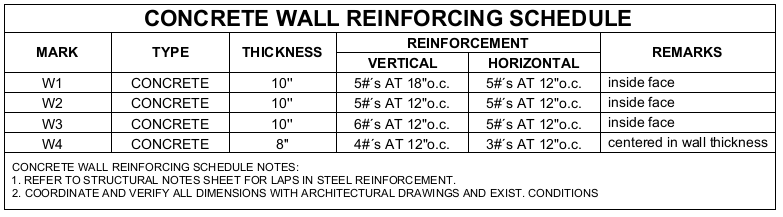
\includegraphics[width=\linewidth]{figures/concrete_wall_reinforcing_schedule.png}
    \caption{Concrete walls reinforcing schedule}\label{tb_concrete_wall_reinforcing_schedule}
\end{table}

\subsubsection{Wall types}
For analysis purposes we have considered the following wall types:

\begin{center}
  \begin{tabular}{|l|c|}
    \hline
    \textbf{Wall} & \textbf{Stem} \\
    & \textbf{height (m)} \\
    \hline
T1 & 3.15\\
T2 & 2.74\\
T3 & 3.53\\
T4 & 3.12\\
T5 & 2.51\\
T6 & 3.43\\
    \hline
  \end{tabular}
\end{center}

\subsubsection{Internal forces}
The envelope of internal forces envelope for each of the walls are given in tables \ref{tb_def_T1} to \ref{tb_def_T6}.

\begin{table}
\begin{center}
\begin{tabular}{|l|}
\hline
\multicolumn{1}{|c|}{\textsc{T1}}\\
\hline
\begin{tabular}{c|l}
\begin{minipage}{85mm}
\vspace{2mm}
\begin{center}
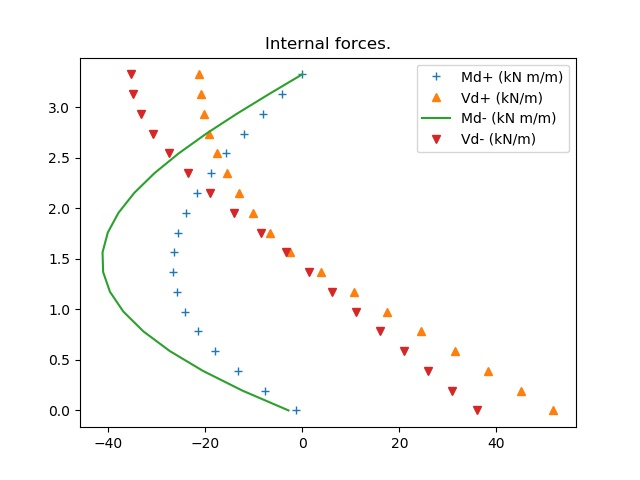
\includegraphics[width=80mm]{figures/T1}
\end{center}
\vspace{1pt}
\end{minipage} & 
\begin{tabular}{l}
\textsc{Wall geometry}\\
Stem top thickness: \\
$b_{top}= 0.25\ m$\\
Stem height: \\
$h_{stem}= 3.15\ m$\\
Stem bottom thickness: \\
$b_{bottom}= 0.25\ m$\\
Footing thickness: \\
$b_{footing}= 0.36\ m$\\
\end{tabular} \\
\end{tabular} \\
\hline
\begin{tabular}{llll}
\multicolumn{3}{c}{\textsc{Materials}}\\
  Concrete: C4000 &   Steel: A615G60 &   Concrete cover: 55 mm\\
\end{tabular} \\
\hline
\end{tabular}
\caption{Wall materials and dimensions T1} \label{tb_def_T1}
\end{center}
\end{table}

\begin{table}
\begin{center}
\begin{tabular}{|l|}
\hline
\multicolumn{1}{|c|}{\textsc{T2}}\\
\hline
\begin{tabular}{c|l}
\begin{minipage}{85mm}
\vspace{2mm}
\begin{center}
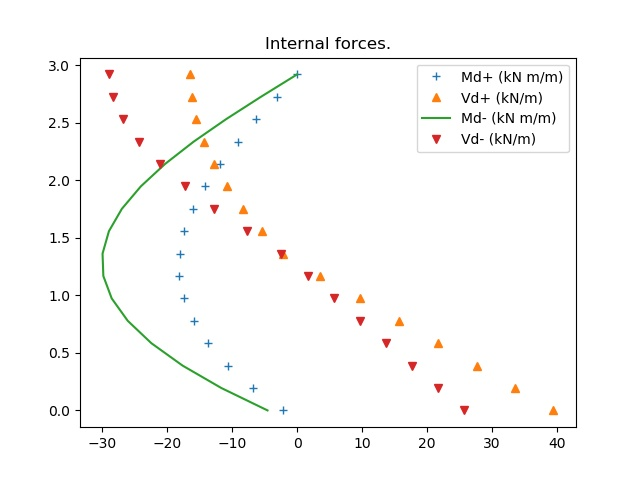
\includegraphics[width=80mm]{figures/T2}
\end{center}
\vspace{1pt}
\end{minipage} & 
\begin{tabular}{l}
\textsc{Wall geometry}\\
Stem top thickness: \\
$b_{top}= 0.25\ m$\\
Stem height: \\
$h_{stem}= 2.74\ m$\\
Stem bottom thickness: \\
$b_{bottom}= 0.25\ m$\\
Footing thickness: \\
$b_{footing}= 0.36\ m$\\
\end{tabular} \\
\end{tabular} \\
\hline
\begin{tabular}{llll}
\multicolumn{3}{c}{\textsc{Materials}}\\
  Concrete: C4000 &   Steel: A615G60 &   Concrete cover: 55 mm\\
\end{tabular} \\
\hline
\end{tabular}
\caption{Wall materials and dimensions T2} \label{tb_def_T2}
\end{center}
\end{table}


\begin{table}
\begin{center}
\begin{tabular}{|l|}
\hline
\multicolumn{1}{|c|}{\textsc{T3}}\\
\hline
\begin{tabular}{c|l}
\begin{minipage}{85mm}
\vspace{2mm}
\begin{center}
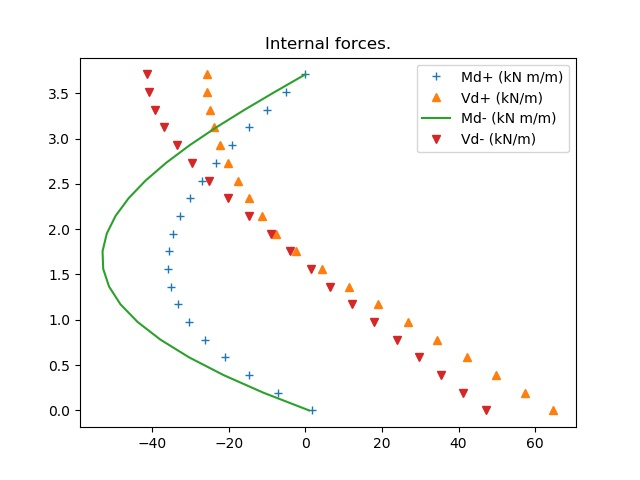
\includegraphics[width=80mm]{figures/T3}
\end{center}
\vspace{1pt}
\end{minipage} & 
\begin{tabular}{l}
\textsc{Wall geometry}\\
Stem top thickness: \\
$b_{top}= 0.25\ m$\\
Stem height: \\
$h_{stem}= 3.53\ m$\\
Stem bottom thickness: \\
$b_{bottom}= 0.25\ m$\\
Footing thickness: \\
$b_{footing}= 0.36\ m$\\
\end{tabular} \\
\end{tabular} \\
\hline
\begin{tabular}{llll}
\multicolumn{3}{c}{\textsc{Materials}}\\
  Concrete: C4000 &   Steel: A615G60 &   Concrete cover: 55 mm\\
\end{tabular} \\
\hline
\end{tabular}
\caption{Wall materials and dimensions T3} \label{tb_def_T3}
\end{center}
\end{table}



\begin{table}
\begin{center}
\begin{tabular}{|l|}
\hline
\multicolumn{1}{|c|}{\textsc{T4}}\\
\hline
\begin{tabular}{c|l}
\begin{minipage}{85mm}
\vspace{2mm}
\begin{center}
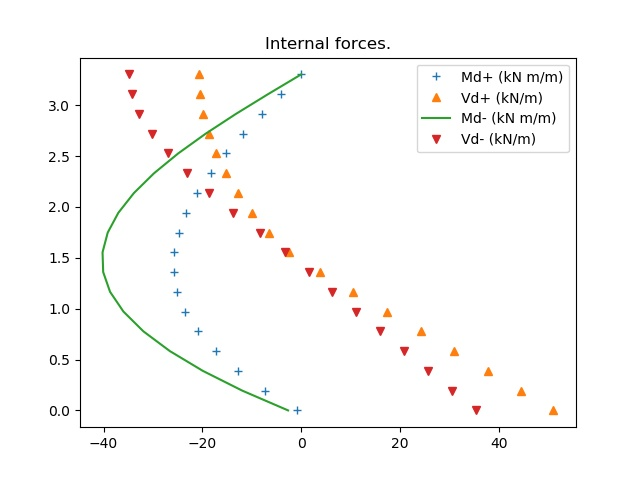
\includegraphics[width=80mm]{figures/T4}
\end{center}
\vspace{1pt}
\end{minipage} & 
\begin{tabular}{l}
\textsc{Wall geometry}\\
Stem top thickness: \\
$b_{top}= 0.25\ m$\\
Stem height: \\
$h_{stem}= 3.12\ m$\\
Stem bottom thickness: \\
$b_{bottom}= 0.25\ m$\\
Footing thickness: \\
$b_{footing}= 0.36\ m$\\
\end{tabular} \\
\end{tabular} \\
\hline
\begin{tabular}{llll}
\multicolumn{3}{c}{\textsc{Materials}}\\
  Concrete: C4000 &   Steel: A615G60 &   Concrete cover: 55 mm\\
\end{tabular} \\
\hline
\end{tabular}
\caption{Wall materials and dimensions T4} \label{tb_def_T4}
\end{center}
\end{table}

\begin{table}
\begin{center}
\begin{tabular}{|l|}
\hline
\multicolumn{1}{|c|}{\textsc{T5}}\\
\hline
\begin{tabular}{c|l}
\begin{minipage}{85mm}
\vspace{2mm}
\begin{center}
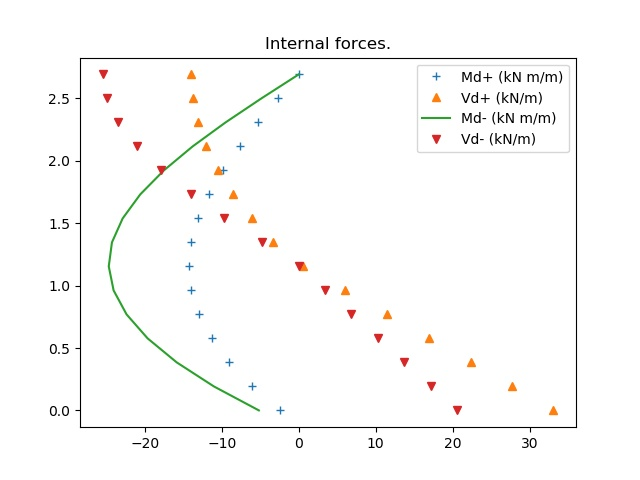
\includegraphics[width=80mm]{figures/T5}
\end{center}
\vspace{1pt}
\end{minipage} & 
\begin{tabular}{l}
\textsc{Wall geometry}\\
Stem top thickness: \\
$b_{top}= 0.25\ m$\\
Stem height: \\
$h_{stem}= 2.51\ m$\\
Stem bottom thickness: \\
$b_{bottom}= 0.25\ m$\\
Footing thickness: \\
$b_{footing}= 0.36\ m$\\
\end{tabular} \\
\end{tabular} \\
\hline
\begin{tabular}{llll}
\multicolumn{3}{c}{\textsc{Materials}}\\
  Concrete: C4000 &   Steel: A615G60 &   Concrete cover: 55 mm\\
\end{tabular} \\
\hline
\end{tabular}
\caption{Wall materials and dimensions T5} \label{tb_def_T5}
\end{center}
\end{table}


\begin{table}
\begin{center}
\begin{tabular}{|l|}
\hline
\multicolumn{1}{|c|}{\textsc{T6}}\\
\hline
\begin{tabular}{c|l}
\begin{minipage}{85mm}
\vspace{2mm}
\begin{center}
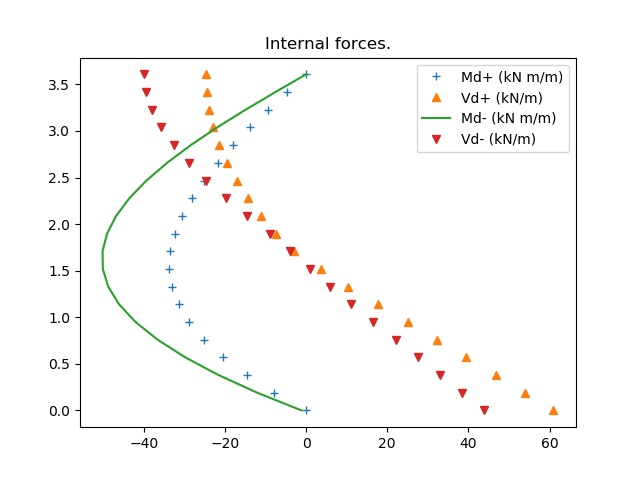
\includegraphics[width=80mm]{figures/T6}
\end{center}
\vspace{1pt}
\end{minipage} & 
\begin{tabular}{l}
\textsc{Wall geometry}\\
Stem top thickness: \\
$b_{top}= 0.25\ m$\\
Stem height: \\
$h_{stem}= 3.43\ m$\\
Stem bottom thickness: \\
$b_{bottom}= 0.25\ m$\\
Footing thickness: \\
$b_{footing}= 0.36\ m$\\
\end{tabular} \\
\end{tabular} \\
\hline
\begin{tabular}{llll}
\multicolumn{3}{c}{\textsc{Materials}}\\
  Concrete: C4000 &   Steel: A615G60 &   Concrete cover: 55 mm\\
\end{tabular} \\
\hline
\end{tabular}
\caption{Wall materials and dimensions T6} \label{tb_def_T6}
\end{center}
\end{table}

\subsubsection{Reinforcement checks}

\tablefirsthead{\hline
\multicolumn{1}{|c|}{\textsc{Wall vertical reinforcements}}\\\hline
}
\tablehead{\hline
\multicolumn{1}{|c|}{\textsc{wall vertical reinforcements (cont.)}}\\\hline
}
\tabletail{\hline \multicolumn{1}{|r|}{../..}\\\hline}
\tablelasttail{\hline}
\begin{center}
\begin{supertabular}{|l|}
\hline
\textbf{T1 wall. Inside stem reinforcement:}\\
  RC section dimensions; b= 1.00 m, h= 0.25 m\\
  diam: 16 mm, spacing: 300 mm  reinf. development L=0.34 m (22 diameters).\\
  area: As=   6.67 cm2/m areaMin:   4.56 cm2/m  F(As)= 1.46 OK!\\
  Bending check: Md=  40.09 kN m, MR=  41.36kN m  F(M)= 1.03 OK!\\
  Shear check: Vd=   7.61 kN,  VR= 199.37 kN  F(V)= 26.21 OK!\\
  %% Stress check: M=  40.09 kN m, $\sigma_s$= 263.03 MPa\\
  %%   $\sigma_{lim}$= 300.00 MPa  F($\sigma_s$)= 1.14 OK!\\
\hline
\textbf{T2 wall. Inside stem reinforcement:}\\
  RC section dimensions; b= 1.00 m, h= 0.25 m\\
  diam: 16 mm, spacing: 400 mm  reinf. development L=0.34 m (22 diameters).\\
  area: As=   5.00 cm2/m areaMin:   4.56 cm2/m  F(As)= 1.10 OK!\\
  Bending check: Md=  29.02 kN m, MR=  31.02kN m  F(M)= 1.07 OK!\\
  Shear check: Vd=   6.84 kN,  VR= 199.37 kN  F(V)= 29.15 OK!\\
  %% Stress check: M=  29.02 kN m, $\sigma_s$= 253.88 MPa\\
  %%   $\sigma_{lim}$= 300.00 MPa  F($\sigma_s$)= 1.18 OK!\\
\hline
\textbf{T3 wall. Inside stem reinforcement:}\\
  RC section dimensions; b= 1.00 m, h= 0.25 m\\
  diam: 19 mm, spacing: 300 mm  reinf. development L=0.61 m (32 diameters).\\
  area: As=   9.47 cm2/m areaMin:   4.56 cm2/m  F(As)= 2.08 OK!\\
  Bending check: Md=  51.88 kN m, MR=  58.26kN m  F(M)= 1.12 OK!\\
  Shear check: Vd=   7.98 kN,  VR= 199.37 kN  F(V)= 24.98 OK!\\
  %% Stress check: M=  51.88 kN m, $\sigma_s$= 239.75 MPa\\
  %%   $\sigma_{lim}$= 300.00 MPa  F($\sigma_s$)= 1.25 $\sim$ OK!\\
\hline
\textbf{T4 wall. Inside stem reinforcement:}\\
  RC section dimensions; b= 1.00 m, h= 0.25 m\\
  diam: 16 mm, spacing: 300 mm  reinf. development L=0.34 m (22 diameters).\\
  area: As=   6.67 cm2/m areaMin:   4.56 cm2/m  F(As)= 1.46 OK!\\
  Bending check: Md=  39.19 kN m, MR=  41.36kN m  F(M)= 1.06 OK!\\
  Shear check: Vd=   7.46 kN,  VR= 199.37 kN  F(V)= 26.73 OK!\\
  %% Stress check: M=  39.19 kN m, $\sigma_s$= 257.14 MPa\\
  %%   $\sigma_{lim}$= 300.00 MPa  F($\sigma_s$)= 1.17 OK!\\
\hline
\textbf{T5 wall. Inside stem reinforcement:}\\
  RC section dimensions; b= 1.00 m, h= 0.25 m\\
  diam: 16 mm, spacing: 400 mm  reinf. development L=0.34 m (22 diameters).\\
  area: As=   5.00 cm2/m areaMin:   4.56 cm2/m  F(As)= 1.10 OK!\\
  Bending check: Md=  23.62 kN m, MR=  31.02kN m  F(M)= 1.31 OK!\\
  Shear check: Vd=   6.42 kN,  VR= 199.37 kN  F(V)= 31.05 OK!\\
  %% Stress check: M=  23.62 kN m, $\sigma_s$= 206.69 MPa\\
  %%   $\sigma_{lim}$= 300.00 MPa  F($\sigma_s$)= 1.45 OK!\\
\hline
\textbf{T6 wall. Inside stem reinforcement:}\\
  RC section dimensions; b= 1.00 m, h= 0.25 m\\
  diam: 19 mm, spacing: 300 mm  reinf. development L=0.61 m (32 diameters).\\
  area: As=   9.47 cm2/m areaMin:   4.56 cm2/m  F(As)= 2.08 OK!\\
  Bending check: Md=  49.02 kN m, MR=  58.26kN m  F(M)= 1.19 OK!\\
  Shear check: Vd=   8.13 kN,  VR= 199.37 kN  F(V)= 24.54 OK!\\
  %% Stress check: M=  49.02 kN m, $\sigma_s$= 226.52 MPa\\
  %%   $\sigma_{lim}$= 300.00 MPa  F($\sigma_s$)= 1.32 OK!\\
\end{supertabular}
\end{center}

\tablefirsthead{\hline
\multicolumn{1}{|c|}{\textsc{Shear check}}\\\hline
}
\tablehead{\hline
\multicolumn{1}{|c|}{\textsc{shear check (cont.)}}\\\hline
}
\tabletail{\hline \multicolumn{1}{|r|}{../..}\\\hline}
\tablelasttail{\hline}
\begin{center}
\begin{supertabular}{|l|}
\textbf{T1 wall. Shear check:}\\
  Shear check: Vd=  42.99 kN,  VR= 199.37 kN  F(V)= 4.64 OK!\\
\hline
\textbf{T2 wall. Shear check:}\\
  Shear check: Vd=  31.78 kN,  VR= 199.37 kN  F(V)= 6.27 OK!\\
\hline
\textbf{T3 wall. Shear check:}\\
  Shear check: Vd=  55.00 kN,  VR= 199.37 kN  F(V)= 3.63 OK!\\
\hline
\textbf{T4 wall. Shear check:}\\
  Shear check: Vd=  42.35 kN,  VR= 199.37 kN  F(V)= 4.71 OK!\\
\hline
\textbf{T5 wall. Shear check:}\\
  Shear check: Vd=  26.03 kN,  VR= 199.37 kN  F(V)= 7.66 OK!\\
\hline
\textbf{T6 wall. Shear check:}\\
  Shear check: Vd=  51.43 kN,  VR= 199.37 kN  F(V)= 3.88 OK!\\
\end{supertabular}
\end{center}

\subsubsection{Wall foundations}
The results obtained for the verifications of the footing stability and the soil-bearing capacity. According to the geotechnical report the allowable soil bearing pressure is 3000 psf ($143.64\ kN/m^2$).
\begin{center}
\begin{tabular}{|l|c|c|c|}
\hline
\multicolumn{4}{|c|}{\textsc{wall foundation: T1}}\\
\hline
Verification:  & $F_{disp}$ & $F_{req}$ & Combination\\
\hline
Overturning:  & $\gg 1$ & 1.00 & EQ1609A\\
Sliding:  & 1.23 & 1.00 & EQ1609A\\
Adm. pressure:  & 1.09 & 1.00 & EQ1613B\\
\hline
\multicolumn{4}{|c|}{\textsc{wall foundation: T2}}\\
\hline
Verification:  & $F_{disp}$ & $F_{req}$ & Combination\\
\hline
Overturning:  & $\gg 1$ & 1.00 & EQ1613B\\
Sliding:  & 1.46 & 1.00 & EQ1609A\\
Adm. pressure:  & 1.13 & 1.00 & EQ1613B\\
\hline
\multicolumn{4}{|c|}{\textsc{wall foundattion: T3}}\\
\hline
Verification:  & $F_{disp}$ & $F_{req}$ & Combination\\
\hline
Overturning:  & $\gg 1$ & 1.00 & EQ1609A\\
Sliding:  & 1.13 & 1.00 & EQ1609A\\
Adm. pressure:  & 1.12 & 1.00 & EQ1613B\\
\hline
\multicolumn{4}{|c|}{\textsc{wall foundation: T4}}\\
\hline
Verification:  & $F_{disp}$ & $F_{req}$ & Combination\\
\hline
Overturning:  & $\gg 1$ & 1.00 & EQ1613B\\
Sliding:  & 1.45 & 1.00 & EQ1609A\\
Adm. pressure:  & 1.08 & 1.00 & EQ1613B\\
\hline
\multicolumn{4}{|c|}{\textsc{wall foundation: T5 }}\\
\hline
Verification:  & $F_{disp}$ & $F_{req}$ & Combination\\
\hline
Overturning:  & $\gg 1$ & 1.00 & EQ1613B\\
Sliding:  & 1.69 & 1.00 & EQ1609A\\
Adm. pressure:  & 1.22 & 1.00 & EQ1613B\\
\hline
\multicolumn{4}{|c|}{\textsc{wall foundation: T6}}\\
\hline
Verification:  & $F_{disp}$ & $F_{req}$ & Combination\\
\hline
Overturning:  & $\gg 1$ & 1.00 & EQ1609A\\
Sliding:  & 1.10 & 1.00 & EQ1609A\\
Adm. pressure:  & 1.03 & 1.00 & EQ1613B\\
\hline
\multicolumn{4}{|l|}{$F_{avail.}$: available security.}\\
\multicolumn{4}{|l|}{$F_{req}$: required security.}\\
\hline
\end{tabular}
\end{center}


\newpage
\appendix
\section*{Appendices}
\addcontentsline{toc}{section}{Appendices}
\renewcommand{\thesubsection}{\Alph{subsection}}

\subsection{Loading criteria} \label{loadCrit}

\section{Dead loads}
\begin{table}[h!]
\begin{tabular}{lp{8cm}p{10cm}}
\multicolumn{3}{l}{Materials}\\
& Wood structural panel  & $ 36.0\ \mathrm{pcf} = 5655 \cfrac{\mathrm{newton}}{\mathrm{meter}^3}$ \\
&  Concrete reinforced stone (including gravel)  & $ 150.0\ \mathrm{pcf} = 23563 \cfrac{\mathrm{newton}}{\mathrm{meter}^3}$ \\
& Steel  & $ 489.0\ \mathrm{pcf} = 76816 \cfrac{\mathrm{newton}}{\mathrm{meter}^3}$ \\
& Gypsum crete  & $ 115.0\ \mathrm{pcf} = 18065 \cfrac{\mathrm{newton}}{\mathrm{meter}^3}$ \\

& Gypsum,loose  & $ 70.0\ \mathrm{pcf} = 10996 \cfrac{\mathrm{newton}}{\mathrm{meter}^3}$ \\
& Earth (not submerged) sand and gravel (wet)  & $ 120.0\ \mathrm{pcf} = 18850 \cfrac{\mathrm{newton}}{\mathrm{meter}^3}$ \\
& Water  & $ 62.4\ \mathrm{pcf} = 9802 \cfrac{\mathrm{newton}}{\mathrm{meter}^3}$ \\


\multicolumn{3}{l}{Frame partitions}\\
& Wood or steel studs, $\frac{1}{2}$in gypsum board inside & $8\ \mathrm{psf}= 383 \ \mathrm{pascal}$ \\
& Wood studs, 2x4 unplastered & $4\ \mathrm{psf}=192 \ \mathrm{pascal}$\\
& Wood studs, 2x4 plastered one side & $12\ \mathrm{psf}= 575\ \mathrm{pascal}$\\
& Wood studs, 2x4 plastered two sides & $20\ \mathrm{psf}=958 \ \mathrm{pascal}$\\
& Movable steel partitions &  $4\ \mathrm{psf}=192 \ \mathrm{pascal}$\\
\multicolumn{3}{l}{Frame walls}\\
& Exterior stud wall 2x4 @ 16in, $\frac{5}{8}$ gypsum insulated, $\cfrac{3}{8}$ in siding &  $11\ \mathrm{psf}=526 \ \mathrm{pascal}$\\
& Exterior stud wall 2x6 @ 16in, $\frac{5}{8}$ gypsum insulated, $\cfrac{3}{8}$ in siding &  $12\ \mathrm{psf}=575 \ \mathrm{pascal}$\\
& Exterior stud wall with brick veneer &   $48\ \mathrm{psf}=2298 \ \mathrm{pascal}$\\
& CMU wall 8in &   $60\ \mathrm{psf}=9425 \ \mathrm{pascal}$\\
& Window, glass, frame and sash & $8\ \mathrm{psf}=383 \ \mathrm{pascal}$\\
\multicolumn{3}{l}{Cladding}\\
& Fiber cement panels, large format $38.4\text{in} \times 102\text{in}$ & $3.2\ \mathrm{psf} = 153\ \mathrm{pascal}$ \\
& Fiber cement panels, small scale $9.6\text{in} \times 102\text{in}$ & $3.2\ \mathrm{psf} = 153\ \mathrm{pascal}$ \\
& Perforated metal panel at exterior HVAC location & \\
\multicolumn{3}{l}{Floor truss}\\
& Single chord @ 24in o.c. spacing & $3.2\ \mathrm{psf} = 153\ \mathrm{pascal}$ \\
& Double chord @ 24in o.c. spacing & $4.25\ \mathrm{psf} = 203\ \mathrm{pascal}$ \\
\multicolumn{3}{l}{Sheating}\\
& Roof sheating & $ 3.5\ \mathrm{psf} = 167\ \mathrm{pascal}$ \\
& Floor sheating & $ 2.5\ \mathrm{psf} = 120\ \mathrm{pascal}$ \\
& Ceilings & $ 2.5\ \mathrm{psf} = 120\ \mathrm{pascal}$ \\
& Deck composite sleeperes (3in) &  $9.00\ \mathrm{psf} = 431\ \mathrm{pascal}$ \\
\end{tabular}
\end{table}

\section{Live loads}
\begin{tabular}{p{5cm}p{2.5cm}|p{2.5cm}|p{4cm}}
\textbf{Occupancy or use} & \textbf{Uniform} & \textbf{Concentrated} & \textbf{Notes}\\
\hline
Private rooms and corridors serving them in multifamily dwelling & $ 40.0\ \mathrm{psf} = 1915 \ \mathrm{pascal}$ & - & \emph{IBC-2018 Table 1607.1}  \\
Stairs and exits & $ 100.0\ \mathrm{psf} = 4788 \ \mathrm{pascal}$ & $300\ \mathrm{pound} = 1334\ \mathrm{newton}$ & \emph{IBC-2018 Table 1607.1. Concentrated load on stair treads applied on an area of 2 inches by 2 inches}  \\
Balconies and decks & same as occupancy served & - &  \emph{IBC-2018 Table 1607.1}  \\
Garages (passenger vehicles only) & $ 40.0\ \mathrm{psf} = 1915 \ \mathrm{pascal}$ & - & \emph{IBC-2018 Table 1607.1}  \\
Cornices & $ 60.0\ \mathrm{psf} = 2873 \ \mathrm{pascal}$ & - & \emph{IBC-2018 Table 1607.1}  \\
Elevator machine room and control room grating & - & $300\ \mathrm{pound} = 1334\ \mathrm{newton}$ & \emph{IBC-2018 Table 1607.1.   Concentrated load  applied on an area of 2 inches by 2 inches}\\
Flat roof (not occupiable) + maintenace & $ 20.0\ \mathrm{psf} = 958 \ \mathrm{pascal}$ & $300\ \mathrm{pound} = 1334\ \mathrm{newton}$ & \emph{IBC-2018 Table 1607.1}  \\
Yards and terraces, pedestrians & $ 100.0\ \mathrm{psf} = 4788 \ \mathrm{pascal}$ & - & \emph{IBC-2018 Table 1607.1}  \\
Sidewalks, vehicular driveways and yards, subject to trucking & $ 250.0\ \mathrm{psf} = 11970 \ \mathrm{pascal}$ & $8000\ \mathrm{pound} = 35586\ \mathrm{newton}$ & \emph{IBC-2018 Table 1607.1}  \\
Corridors first floor & $ 100.0\ \mathrm{psf} = 4788 \ \mathrm{pascal}$ & - & \emph{IBC-2018 Table 1607.1}  \\
Store first floor & $ 100.0\ \mathrm{psf} = 4788 \ \mathrm{pascal}$ & - & \emph{IBC-2018 Table 1607.1}  \\

\end{tabular}

\section{Snow loads}
\begin{tabular}{p{5cm}p{5cm}|p{5cm}}
Ground snow load & $p_g = 60.0\ \mathrm{psf} = 2873 \ \mathrm{pascal}$ & \emph{ASCE 7. Figure 7.1}\\
Exposure factor & $C_e = 1.0$ &  \emph{ASCE 7. Table 7-2. Terrain category B, roof partially exposed} \\
Thermal factor &  $C_t = 1.0$ & \emph{ASCE 7. Table 7-3.}\\
Snow load importance factor & $I_s = 1.0$ & \emph{ASCE 7. Table 7-4. Structure risk category II}\\
\textbf{Snow load flat roof} & $p_f = 0.7 \times C_e \times C_t \times  I_s\times p_g = 0.7 \times 1.0 \times 1.0 \times 1.0 \times 60.0 = 42.0\ \mathrm{psf} = 2873 \ \mathrm{pascal}$ & \emph{ASCE 7. Sect. 7.3}\\
\end{tabular}

\section{Wind loads}
\begin{tabular}{p{5cm}l|p{5cm}}
\multicolumn{2}{l|}{Alternate all-heights method.} & \emph{IBC-2018, sect. 1609.6.  Regularly shaped building, less than 75 feet in height, not sensitive to dynamic effects, not channeling effects or buffeting, simple diaphragm building} \\
Ultimate design wind speed & $V_{ult} = 115 \frac{\mathrm{miles}}{\mathrm{hour}} = 51 \frac{\mathrm{meters}}{\mathrm{second}} $& \emph{IBC-2018, figure 1609.3(1). Risk category II building}\\
Velocity pressure exposure coefficient & $K_z = 0.72$ & \emph{ASCE 7, table 27.3.1. Exposure B, height above ground level z $\approx$ 33 feet} \\
Topographic factor & $K_{zt} = 1.0 $ & \emph{ASCE 7, sect. 26.8} \\
\end{tabular}

\vspace{5mm}

\begin{tabular}{lcc|p{5cm}}
\multicolumn{3}{p{8cm}|}{\textbf{Net pressure coefficients $C_{net}$}. Main windforce-resisting frames and systems} & \emph{IBC-2018, Table 1609.6.2, enclosed} \\
Description & $C_{net}$ + Internal & $C_{net}$ - Internal & \\
 & pressure &  presure & \\
 \cline{1-3}
Windward wall & 0.43 & 0.73 & \\
Leeward wall & -0.51 & -0.21 & \\
Sidewall & -0.66 & -0.35 & \\
Parapet windward wall & \multicolumn{2}{c|}{1.28} & \\
Parapet leeward wall & \multicolumn{2}{c|}{-0.85} & \\
Flat roof & -1.09 & -0.79 & \\
\end{tabular}

\vspace{5mm}

\begin{tabular}{lp{4cm}p{4cm}|p{2cm}}
\multicolumn{3}{l|}{\textbf{Design wind pressures $P_{net}$}. Main windforce-resisting frames and systems} & \emph{IBC-2018, sect. 1609.6.3} \\
\multicolumn{3}{p{8cm}|}{$P_{net} = 0.00256 \times V^2 \times K_z \times C_{net} \times K_{zt}$} & \\
Description & $P_{net}$ + Internal & $P_{net}$ - Internal & \\
 & pressure &  presure & \\
 \cline{1-3}
Windward wall & $10.5\ \mathrm{psf} =  501\ \mathrm{pascal}$ & $17.8\ \mathrm{psf} =  852\ \mathrm{pascal}$  & \\
Leeward wall & $-12.4\ \mathrm{psf} =  -595\ \mathrm{pascal}$  & $-5.1\ \mathrm{psf} =  -245\ \mathrm{pascal}$  & \\
Sidewall & $-16.1\ \mathrm{psf} =  -770\ \mathrm{pascal}$  & $-8.5\ \mathrm{psf} =  -409\ \mathrm{pascal}$  & \\
Parapet windward wall & \multicolumn{2}{c|}{$31.2\ \mathrm{psf} =  1494\ \mathrm{pascal}$ } & \\
Parapet leeward wall & \multicolumn{2}{c|}{$-20.7\ \mathrm{psf} =  -992\ \mathrm{pascal}$ } & \\
Flat roof & $-26.6\ \mathrm{psf} =  -1272\ \mathrm{pascal}$  & $-19.3\ \mathrm{psf} =  -992\ \mathrm{pascal}$  & \\
\end{tabular}

\section{Earthquake loads}
\begin{tabular}{p{4cm}l|p{4cm}}
Parameter 0.2-second spectral response acceleration & $S_s = 0.045$ &  \emph{IBC-2018, figure 1613.3.1(1). Site class B} \\
Parameter 1-second spectral response acceleration & $S_1 = 0.038$ &  \emph{IBC-2018, figure 1613.3.1(2). Site class B} \\
Seismic design category & $S_1 \le 0.04\ and\  S_s \le 0.15 \rightarrow $ SDS A & \emph{IBC-2018, sect. 1613.3.1} \\
Site coefficients & $F_a$ = 1.0, $F_v$ = 1.0 & \emph{IBC-2018, tables 1613.3.3(1) and 1613.3.3(2). Site class  B} \\
Maximum considered earthquake spectral response acceleration for short periods & $S_{MS} = F_a\cdot S_s = 0.045$ &  \emph{IBC-2018, sect. 163.3.3} \\
& $S_{M1} = F_a\cdot S_1 = 0.038$ &  \emph{IBC-2018, sect. 163.3.3} \\
Design spectral response acceleration parameters & $S_{DS} = \cfrac{2}{3} S_{MS} = 0.03$ & \emph{IBC-2018, sect. 163.3.4} \\
& $S_{D1} = \cfrac{2}{3} S_{M1} = 0.025$ & \emph{IBC-2018, sect. 163.3.4} \\
\end{tabular}

\end{document}


\newpage
\subsection{Calculation results. Internal forces on columns}\label{sc_column_internal_forces}
\subsubsection{Ultimate limit states}
\begin{figure}
\begin{center}
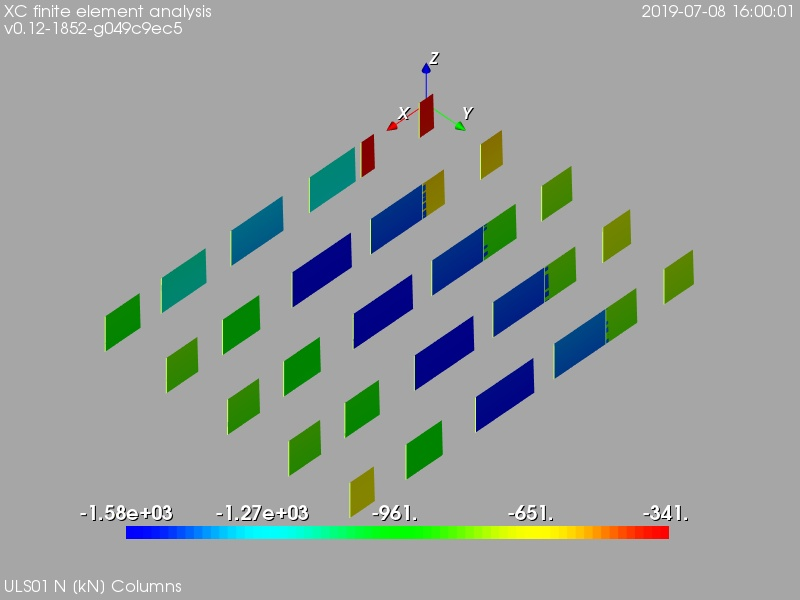
\includegraphics[width=75mm]{annex_res_columns/graphics/resSimplLC/ULS01columnsN}
\caption{ULS01: 1.4*D. Columns, internal axial force [kN]}
\end{center}
\end{figure}
\begin{figure}
\begin{center}
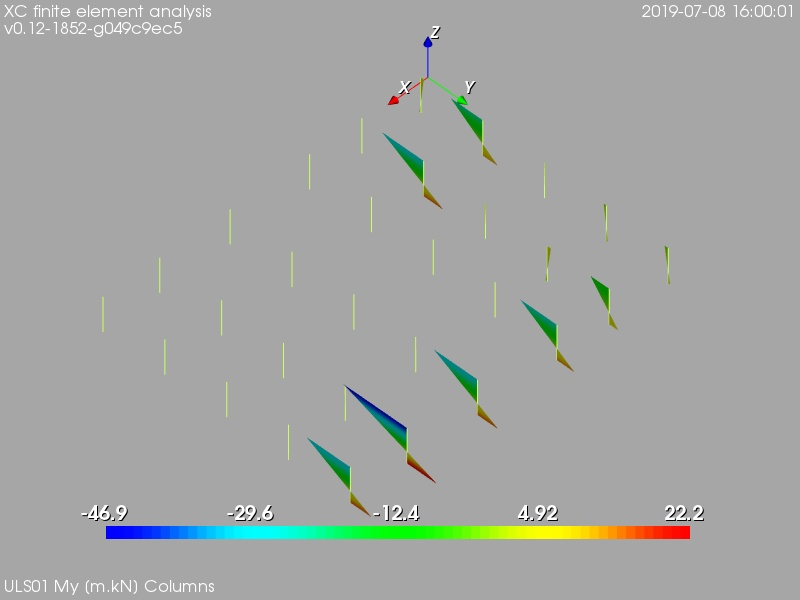
\includegraphics[width=75mm]{annex_res_columns/graphics/resSimplLC/ULS01columnsMy}
\caption{ULS01: 1.4*D. Columns, bending moment about local axis y [m.kN]}
\end{center}
\end{figure}
\begin{figure}
\begin{center}
\includegraphics[width=75mm]{annex_res_columns/graphics/resSimplLC/ULS01columnsMz}
\caption{ULS01: 1.4*D. Columns, bending moment about local axis z [m.kN]}
\end{center}
\end{figure}
\begin{figure}
\begin{center}
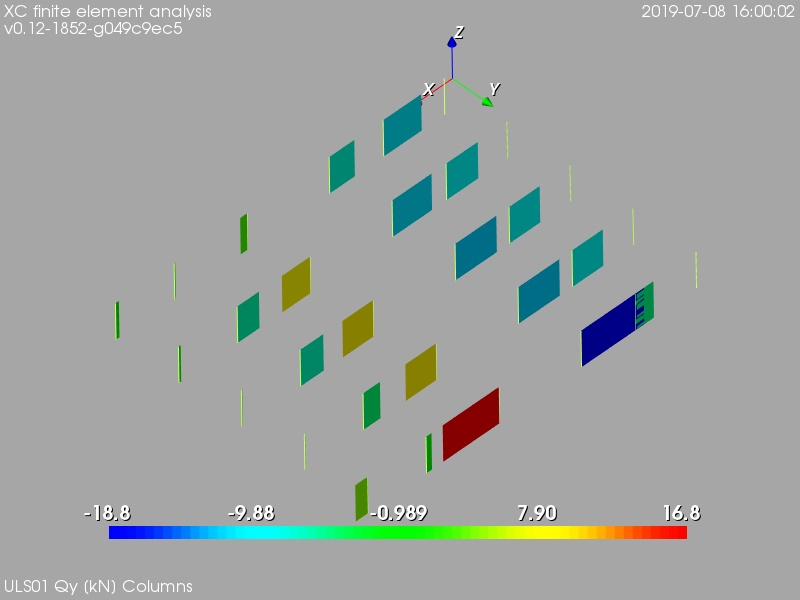
\includegraphics[width=75mm]{annex_res_columns/graphics/resSimplLC/ULS01columnsQy}
\caption{ULS01: 1.4*D. Columns, internal shear force in local direction y [kN]}
\end{center}
\end{figure}
\begin{figure}

\begin{center}
\includegraphics[width=75mm]{annex_res_columns/graphics/resSimplLC/ULS01columnsQz}
\caption{ULS01: 1.4*D. Columns, internal shear force in local direction z [kN]}
\end{center}
\end{figure}

\begin{figure}
\begin{center}
\includegraphics[width=75mm]{annex_res_columns/graphics/resSimplLC/ULS02_acolumnsN}
\caption{ULS02\_a: 1.2*D + 1.6*Lru + Lpu + 0.5*S. Columns, internal axial force [kN]}
\end{center}
\end{figure}
\begin{figure}
\begin{center}
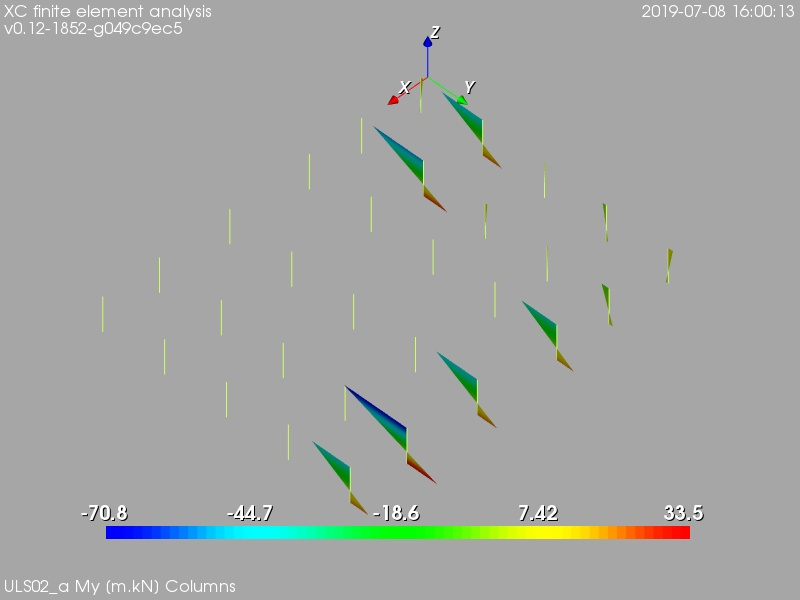
\includegraphics[width=75mm]{annex_res_columns/graphics/resSimplLC/ULS02_acolumnsMy}
\caption{ULS02\_a: 1.2*D + 1.6*Lru + Lpu + 0.5*S. Columns, bending moment about local axis y [m.kN]}
\end{center}
\end{figure}
\begin{figure}
\begin{center}
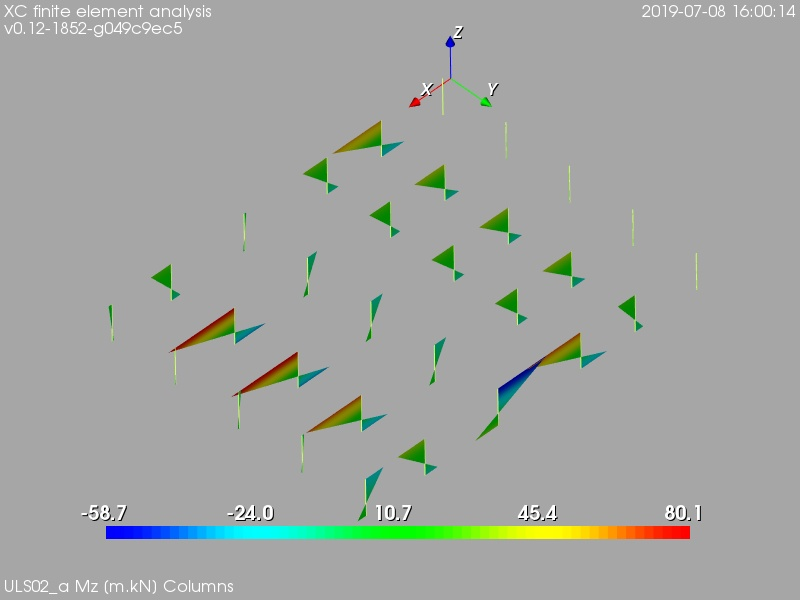
\includegraphics[width=75mm]{annex_res_columns/graphics/resSimplLC/ULS02_acolumnsMz}
\caption{ULS02\_a: 1.2*D + 1.6*Lru + Lpu + 0.5*S. Columns, bending moment about local axis z [m.kN]}
\end{center}
\end{figure}
\begin{figure}
\begin{center}
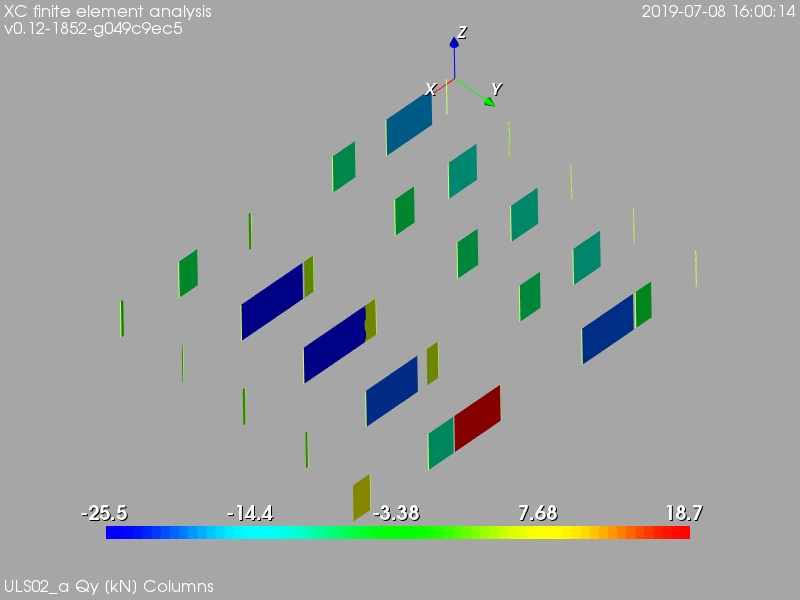
\includegraphics[width=75mm]{annex_res_columns/graphics/resSimplLC/ULS02_acolumnsQy}
\caption{ULS02\_a: 1.2*D + 1.6*Lru + Lpu + 0.5*S. Columns, internal shear force in local direction y [kN]}
\end{center}
\end{figure}
\begin{figure}
\begin{center}
\includegraphics[width=75mm]{annex_res_columns/graphics/resSimplLC/ULS02_acolumnsQz}
\caption{ULS02\_a: 1.2*D + 1.6*Lru + Lpu + 0.5*S. Columns, internal shear force in local direction z [kN]}
\end{center}
\end{figure}

\begin{figure}
\begin{center}
\includegraphics[width=75mm]{annex_res_columns/graphics/resSimplLC/ULS02_bcolumnsN}
\caption{ULS02\_b: 1.2*D + 1.6*Lrs + Lps + 0.5*S. Columns, internal axial force [kN]}
\end{center}
\end{figure}
\begin{figure}
\begin{center}
\includegraphics[width=75mm]{annex_res_columns/graphics/resSimplLC/ULS02_bcolumnsMy}
\caption{ULS02\_b: 1.2*D + 1.6*Lrs + Lps + 0.5*S. Columns, bending moment about local axis y [m.kN]}
\end{center}
\end{figure}
\begin{figure}
\begin{center}
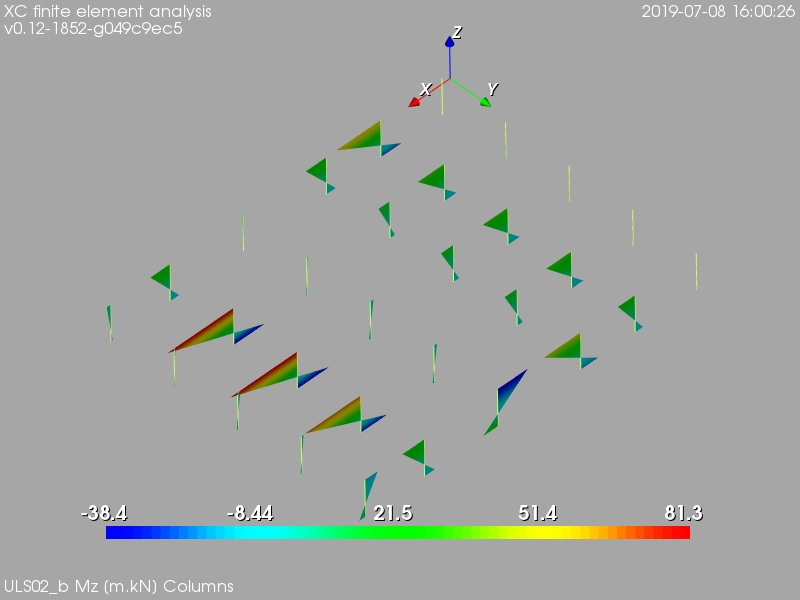
\includegraphics[width=75mm]{annex_res_columns/graphics/resSimplLC/ULS02_bcolumnsMz}
\caption{ULS02\_b: 1.2*D + 1.6*Lrs + Lps + 0.5*S. Columns, bending moment about local axis z [m.kN]}
\end{center}
\end{figure}
\begin{figure}
\begin{center}
\includegraphics[width=75mm]{annex_res_columns/graphics/resSimplLC/ULS02_bcolumnsQy}
\caption{ULS02\_b: 1.2*D + 1.6*Lrs + Lps + 0.5*S. Columns, internal shear force in local direction y [kN]}
\end{center}
\end{figure}
\begin{figure}
\begin{center}
\includegraphics[width=75mm]{annex_res_columns/graphics/resSimplLC/ULS02_bcolumnsQz}
\caption{ULS02\_b: 1.2*D + 1.6*Lrs + Lps + 0.5*S. Columns, internal shear force in local direction z [kN]}
\end{center}
\end{figure}

\begin{figure}
\begin{center}
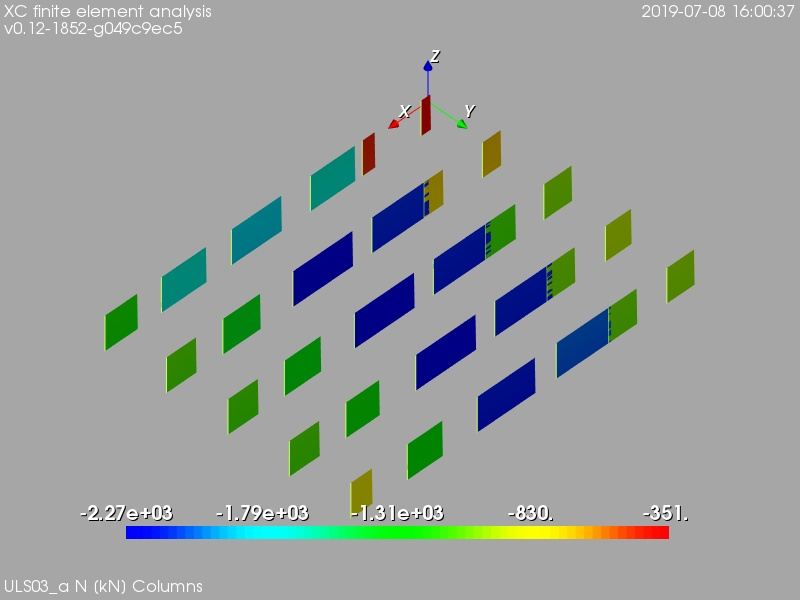
\includegraphics[width=75mm]{annex_res_columns/graphics/resSimplLC/ULS03_acolumnsN}
\caption{ULS03\_a: 1.2*D + 1.6*S + 0.5*Lru + Lpu. Columns, internal axial force [kN]}
\end{center}
\end{figure}
\begin{figure}
\begin{center}
\includegraphics[width=75mm]{annex_res_columns/graphics/resSimplLC/ULS03_acolumnsMy}
\caption{ULS03\_a: 1.2*D + 1.6*S + 0.5*Lru + Lpu. Columns, bending moment about local axis y [m.kN]}
\end{center}
\end{figure}
\begin{figure}
\begin{center}
\includegraphics[width=75mm]{annex_res_columns/graphics/resSimplLC/ULS03_acolumnsMz}
\caption{ULS03\_a: 1.2*D + 1.6*S + 0.5*Lru + Lpu. Columns, bending moment about local axis z [m.kN]}
\end{center}
\end{figure}
\begin{figure}
\begin{center}

\includegraphics[width=75mm]{annex_res_columns/graphics/resSimplLC/ULS03_acolumnsQy}
\caption{ULS03\_a: 1.2*D + 1.6*S + 0.5*Lru + Lpu. Columns, internal shear force in local direction y [kN]}
\end{center}
\end{figure}
\begin{figure}
\begin{center}
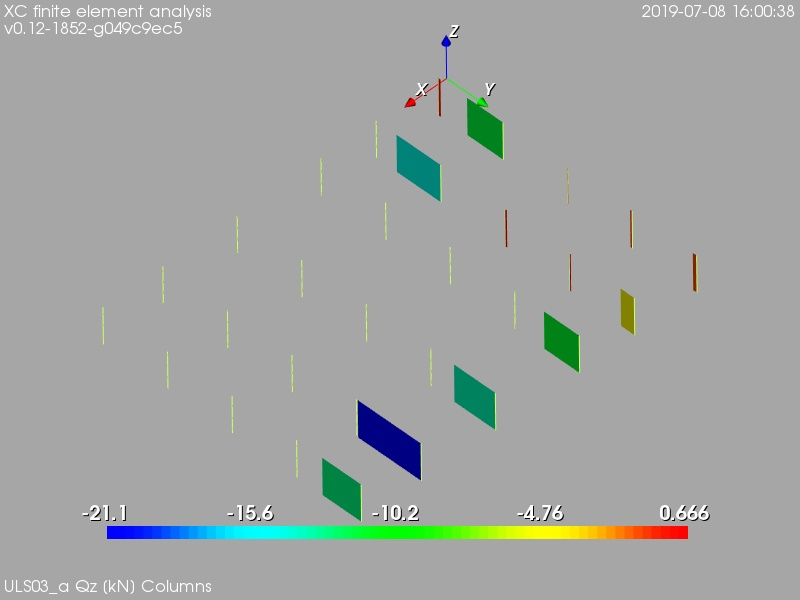
\includegraphics[width=75mm]{annex_res_columns/graphics/resSimplLC/ULS03_acolumnsQz}
\caption{ULS03\_a: 1.2*D + 1.6*S + 0.5*Lru + Lpu. Columns, internal shear force in local direction z [kN]}
\end{center}
\end{figure}

\begin{figure}
\begin{center}
\includegraphics[width=75mm]{annex_res_columns/graphics/resSimplLC/ULS03_bcolumnsN}
\caption{ULS03\_b: 1.2*D + 1.6*S + 0.5*Lrs + Lps. Columns, internal axial force [kN]}
\end{center}
\end{figure}
\begin{figure}
\begin{center}
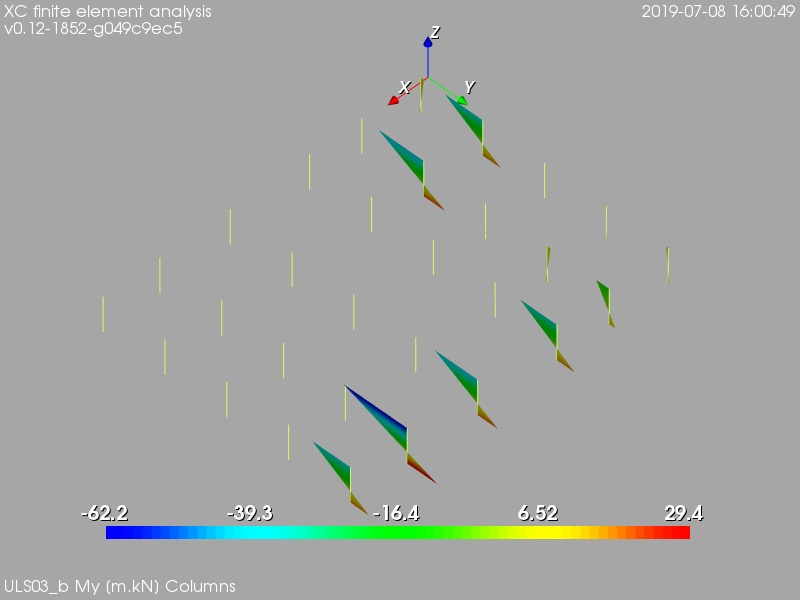
\includegraphics[width=75mm]{annex_res_columns/graphics/resSimplLC/ULS03_bcolumnsMy}
\caption{ULS03\_b: 1.2*D + 1.6*S + 0.5*Lrs + Lps. Columns, bending moment about local axis y [m.kN]}
\end{center}
\end{figure}
\begin{figure}
\begin{center}
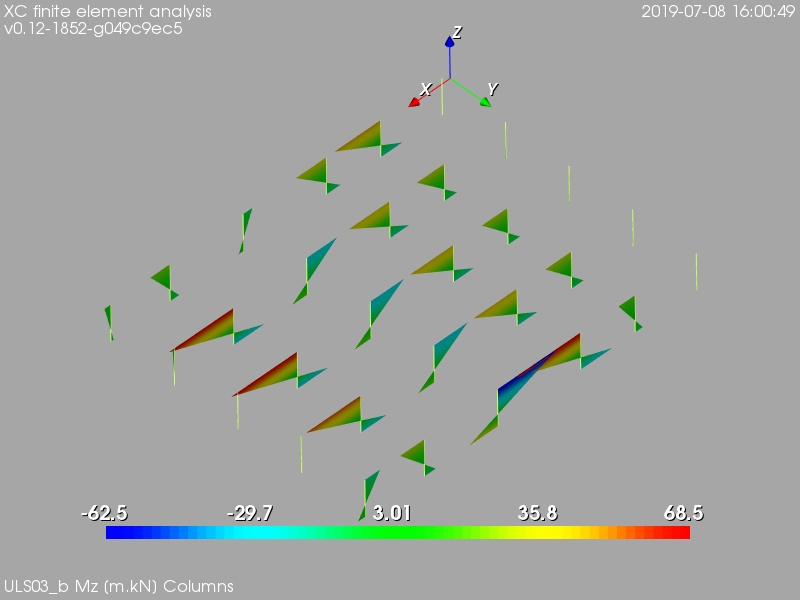
\includegraphics[width=75mm]{annex_res_columns/graphics/resSimplLC/ULS03_bcolumnsMz}
\caption{ULS03\_b: 1.2*D + 1.6*S + 0.5*Lrs + Lps. Columns, bending moment about local axis z [m.kN]}
\end{center}
\end{figure}
\begin{figure}
\begin{center}
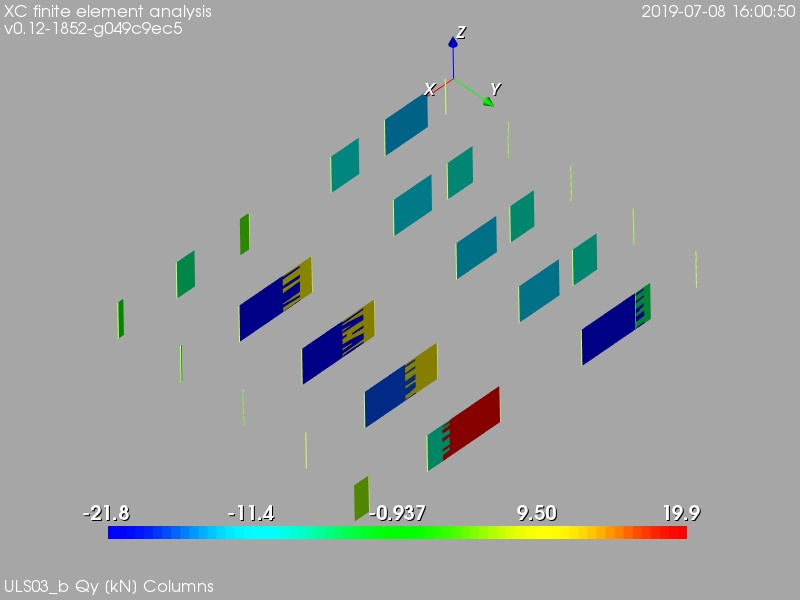
\includegraphics[width=75mm]{annex_res_columns/graphics/resSimplLC/ULS03_bcolumnsQy}
\caption{ULS03\_b: 1.2*D + 1.6*S + 0.5*Lrs + Lps. Columns, internal shear force in local direction y [kN]}
\end{center}
\end{figure}
\begin{figure}
\begin{center}
\includegraphics[width=75mm]{annex_res_columns/graphics/resSimplLC/ULS03_bcolumnsQz}
\caption{ULS03\_b: 1.2*D + 1.6*S + 0.5*Lrs + Lps. Columns, internal shear force in local direction z [kN]}
\end{center}
\end{figure}

\begin{figure}
\begin{center}
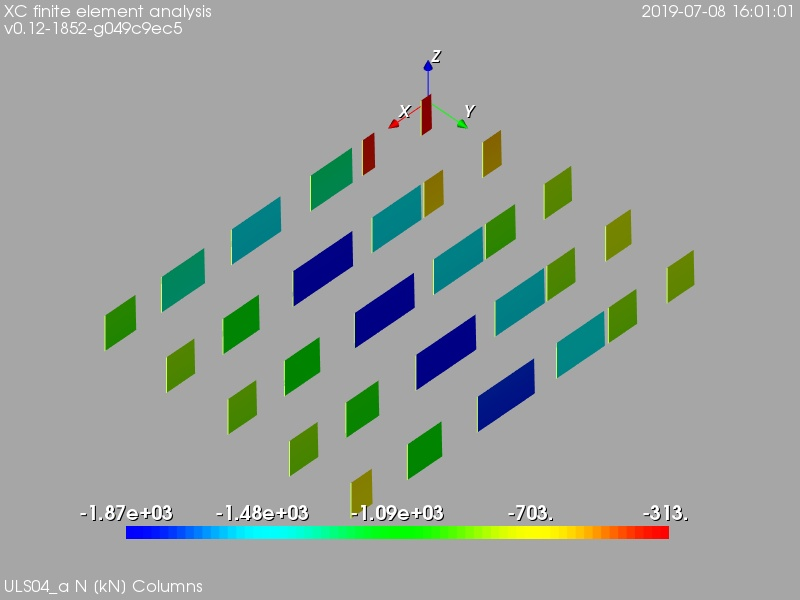
\includegraphics[width=75mm]{annex_res_columns/graphics/resSimplLC/ULS04_acolumnsN}
\caption{ULS04\_a: 1.2*D + 1.6*S + 0.5*W\_WE. Columns, internal axial force [kN]}
\end{center}
\end{figure}
\begin{figure}
\begin{center}
\includegraphics[width=75mm]{annex_res_columns/graphics/resSimplLC/ULS04_acolumnsMy}
\caption{ULS04\_a: 1.2*D + 1.6*S + 0.5*W\_WE. Columns, bending moment about local axis y [m.kN]}
\end{center}
\end{figure}
\begin{figure}
\begin{center}
\includegraphics[width=75mm]{annex_res_columns/graphics/resSimplLC/ULS04_acolumnsMz}
\caption{ULS04\_a: 1.2*D + 1.6*S + 0.5*W\_WE. Columns, bending moment about local axis z [m.kN]}
\end{center}
\end{figure}

\begin{figure}
\begin{center}
\includegraphics[width=75mm]{annex_res_columns/graphics/resSimplLC/ULS04_acolumnsQy}
\caption{ULS04\_a: 1.2*D + 1.6*S + 0.5*W\_WE. Columns, internal shear force in local direction y [kN]}
\end{center}
\end{figure}
\begin{figure}
\begin{center}
\includegraphics[width=75mm]{annex_res_columns/graphics/resSimplLC/ULS04_acolumnsQz}
\caption{ULS04\_a: 1.2*D + 1.6*S + 0.5*W\_WE. Columns, internal shear force in local direction z [kN]}
\end{center}
\end{figure}

\begin{figure}
\begin{center}
\includegraphics[width=75mm]{annex_res_columns/graphics/resSimplLC/ULS04_bcolumnsN}
\caption{ULS04\_b: 1.2*D + 1.6*S + 0.5*W\_NS. Columns, internal axial force [kN]}
\end{center}
\end{figure}
\begin{figure}
\begin{center}
\includegraphics[width=75mm]{annex_res_columns/graphics/resSimplLC/ULS04_bcolumnsMy}
\caption{ULS04\_b: 1.2*D + 1.6*S + 0.5*W\_NS. Columns, bending moment about local axis y [m.kN]}
\end{center}
\end{figure}
\begin{figure}
\begin{center}
\includegraphics[width=75mm]{annex_res_columns/graphics/resSimplLC/ULS04_bcolumnsMz}
\caption{ULS04\_b: 1.2*D + 1.6*S + 0.5*W\_NS. Columns, bending moment about local axis z [m.kN]}
\end{center}
\end{figure}
\begin{figure}
\begin{center}
\includegraphics[width=75mm]{annex_res_columns/graphics/resSimplLC/ULS04_bcolumnsQy}
\caption{ULS04\_b: 1.2*D + 1.6*S + 0.5*W\_NS. Columns, internal shear force in local direction y [kN]}
\end{center}
\end{figure}
\begin{figure}
\begin{center}
\includegraphics[width=75mm]{annex_res_columns/graphics/resSimplLC/ULS04_bcolumnsQz}
\caption{ULS04\_b: 1.2*D + 1.6*S + 0.5*W\_NS. Columns, internal shear force in local direction z [kN]}
\end{center}
\end{figure}

\begin{figure}
\begin{center}
\includegraphics[width=75mm]{annex_res_columns/graphics/resSimplLC/ULS05_acolumnsN}
\caption{ULS05\_a: 1.2*D + W\_WE + 0.5*Lru + Lpu. Columns, internal axial force [kN]}
\end{center}
\end{figure}
\begin{figure}
\begin{center}
\includegraphics[width=75mm]{annex_res_columns/graphics/resSimplLC/ULS05_acolumnsMy}
\caption{ULS05\_a: 1.2*D + W\_WE + 0.5*Lru + Lpu. Columns, bending moment about local axis y [m.kN]}
\end{center}
\end{figure}
\begin{figure}
\begin{center}
\includegraphics[width=75mm]{annex_res_columns/graphics/resSimplLC/ULS05_acolumnsMz}
\caption{ULS05\_a: 1.2*D + W\_WE + 0.5*Lru + Lpu. Columns, bending moment about local axis z [m.kN]}
\end{center}
\end{figure}
\begin{figure}
\begin{center}
\includegraphics[width=75mm]{annex_res_columns/graphics/resSimplLC/ULS05_acolumnsQy}
\caption{ULS05\_a: 1.2*D + W\_WE + 0.5*Lru + Lpu. Columns, internal shear force in local direction y [kN]}
\end{center}
\end{figure}
\begin{figure}
\begin{center}
\includegraphics[width=75mm]{annex_res_columns/graphics/resSimplLC/ULS05_acolumnsQz}
\caption{ULS05\_a: 1.2*D + W\_WE + 0.5*Lru + Lpu. Columns, internal shear force in local direction z [kN]}
\end{center}
\end{figure}
% Hasta aquí bien
\clearpage
\begin{figure}
\begin{center}
\includegraphics[width=75mm]{annex_res_columns/graphics/resSimplLC/ULS05_bcolumnsN}
\caption{ULS05\_b: 1.2*D + W\_NS + 0.5*Lru + Lpu. Columns, internal axial force [kN]}
\end{center}
\end{figure}
\begin{figure}
\begin{center}
\includegraphics[width=75mm]{annex_res_columns/graphics/resSimplLC/ULS05_bcolumnsMy}
\caption{ULS05\_b: 1.2*D + W\_NS + 0.5*Lru + Lpu. Columns, bending moment about local axis y [m.kN]}
\end{center}
\end{figure}
\begin{figure}
\begin{center}
\includegraphics[width=75mm]{annex_res_columns/graphics/resSimplLC/ULS05_bcolumnsMz}
\caption{ULS05\_b: 1.2*D + W\_NS + 0.5*Lru + Lpu. Columns, bending moment about local axis z [m.kN]}
\end{center}
\end{figure}
\begin{figure}
\begin{center}
\includegraphics[width=75mm]{annex_res_columns/graphics/resSimplLC/ULS05_bcolumnsQy}
\caption{ULS05\_b: 1.2*D + W\_NS + 0.5*Lru + Lpu. Columns, internal shear force in local direction y [kN]}
\end{center}
\end{figure}
\begin{figure}
\begin{center}
\includegraphics[width=75mm]{annex_res_columns/graphics/resSimplLC/ULS05_bcolumnsQz}
\caption{ULS05\_b: 1.2*D + W\_NS + 0.5*Lru + Lpu. Columns, internal shear force in local direction z [kN]}
\end{center}
\end{figure}


\begin{figure}
\begin{center}
\includegraphics[width=75mm]{annex_res_columns/graphics/resSimplLC/ULS05_ccolumnsN}
\caption{ULS05\_c: 1.2*D + W\_WE + 0.5*Lrs + Lps. Columns, internal axial force [kN]}
\end{center}
\end{figure}
\begin{figure}
\begin{center}
\includegraphics[width=75mm]{annex_res_columns/graphics/resSimplLC/ULS05_ccolumnsMy}
\caption{ULS05\_c: 1.2*D + W\_WE + 0.5*Lrs + Lps. Columns, bending moment about local axis y [m.kN]}
\end{center}
\end{figure}
\begin{figure}
\begin{center}
\includegraphics[width=75mm]{annex_res_columns/graphics/resSimplLC/ULS05_ccolumnsMz}
\caption{ULS05\_c: 1.2*D + W\_WE + 0.5*Lrs + Lps. Columns, bending moment about local axis z [m.kN]}
\end{center}
\end{figure}
\begin{figure}
\begin{center}
\includegraphics[width=75mm]{annex_res_columns/graphics/resSimplLC/ULS05_ccolumnsQy}
\caption{ULS05\_c: 1.2*D + W\_WE + 0.5*Lrs + Lps. Columns, internal shear force in local direction y [kN]}
\end{center}
\end{figure}
\begin{figure}
\begin{center}
\includegraphics[width=75mm]{annex_res_columns/graphics/resSimplLC/ULS05_ccolumnsQz}
\caption{ULS05\_c: 1.2*D + W\_WE + 0.5*Lrs + Lps. Columns, internal shear force in local direction z [kN]}
\end{center}
\end{figure}

\begin{figure}
\begin{center}
\includegraphics[width=75mm]{annex_res_columns/graphics/resSimplLC/ULS05_dcolumnsN}
\caption{ULS05\_d: 1.2*D + W\_NS + 0.5*Lrs + Lps. Columns, internal axial force [kN]}
\end{center}
\end{figure}
\begin{figure}
\begin{center}
\includegraphics[width=75mm]{annex_res_columns/graphics/resSimplLC/ULS05_dcolumnsMy}
\caption{ULS05\_d: 1.2*D + W\_NS + 0.5*Lrs + Lps. Columns, bending moment about local axis y [m.kN]}
\end{center}
\end{figure}
\begin{figure}
\begin{center}
\includegraphics[width=75mm]{annex_res_columns/graphics/resSimplLC/ULS05_dcolumnsMz}
\caption{ULS05\_d: 1.2*D + W\_NS + 0.5*Lrs + Lps. Columns, bending moment about local axis z [m.kN]}
\end{center}
\end{figure}
\begin{figure}
\begin{center}
\includegraphics[width=75mm]{annex_res_columns/graphics/resSimplLC/ULS05_dcolumnsQy}
\caption{ULS05\_d: 1.2*D + W\_NS + 0.5*Lrs + Lps. Columns, internal shear force in local direction y [kN]}
\end{center}
\end{figure}
\begin{figure}
\begin{center}
\includegraphics[width=75mm]{annex_res_columns/graphics/resSimplLC/ULS05_dcolumnsQz}
\caption{ULS05\_d: 1.2*D + W\_NS + 0.5*Lrs + Lps. Columns, internal shear force in local direction z [kN]}
\end{center}
\end{figure}

\begin{figure}
\begin{center}
\includegraphics[width=75mm]{annex_res_columns/graphics/resSimplLC/ULS06_acolumnsN}
\caption{ULS06\_a: 1.2*D + 0.5*Lru + Lpu + 0.2*S. Columns, internal axial force [kN]}
\end{center}
\end{figure}
\begin{figure}
\begin{center}
\includegraphics[width=75mm]{annex_res_columns/graphics/resSimplLC/ULS06_acolumnsMy}
\caption{ULS06\_a: 1.2*D + 0.5*Lru + Lpu + 0.2*S. Columns, bending moment about local axis y [m.kN]}
\end{center}
\end{figure}
\begin{figure}
\begin{center}
\includegraphics[width=75mm]{annex_res_columns/graphics/resSimplLC/ULS06_acolumnsMz}
\caption{ULS06\_a: 1.2*D + 0.5*Lru + Lpu + 0.2*S. Columns, bending moment about local axis z [m.kN]}
\end{center}
\end{figure}
\begin{figure}
\begin{center}
\includegraphics[width=75mm]{annex_res_columns/graphics/resSimplLC/ULS06_acolumnsQy}
\caption{ULS06\_a: 1.2*D + 0.5*Lru + Lpu + 0.2*S. Columns, internal shear force in local direction y [kN]}
\end{center}
\end{figure}
\begin{figure}
\begin{center}
\includegraphics[width=75mm]{annex_res_columns/graphics/resSimplLC/ULS06_acolumnsQz}
\caption{ULS06\_a: 1.2*D + 0.5*Lru + Lpu + 0.2*S. Columns, internal shear force in local direction z [kN]}
\end{center}
\end{figure}

\begin{figure}
\begin{center}
\includegraphics[width=75mm]{annex_res_columns/graphics/resSimplLC/ULS06_bcolumnsN}
\caption{ULS06\_b: 1.2*D + 0.5*Lrs + Lps + 0.2*S. Columns, internal axial force [kN]}
\end{center}
\end{figure}
\begin{figure}
\begin{center}
\includegraphics[width=75mm]{annex_res_columns/graphics/resSimplLC/ULS06_bcolumnsMy}
\caption{ULS06\_b: 1.2*D + 0.5*Lrs + Lps + 0.2*S. Columns, bending moment about local axis y [m.kN]}
\end{center}
\end{figure}
\begin{figure}
\begin{center}
\includegraphics[width=75mm]{annex_res_columns/graphics/resSimplLC/ULS06_bcolumnsMz}
\caption{ULS06\_b: 1.2*D + 0.5*Lrs + Lps + 0.2*S. Columns, bending moment about local axis z [m.kN]}
\end{center}
\end{figure}
\begin{figure}
\begin{center}
\includegraphics[width=75mm]{annex_res_columns/graphics/resSimplLC/ULS06_bcolumnsQy}
\caption{ULS06\_b: 1.2*D + 0.5*Lrs + Lps + 0.2*S. Columns, internal shear force in local direction y [kN]}
\end{center}
\end{figure}
\begin{figure}
\begin{center}
\includegraphics[width=75mm]{annex_res_columns/graphics/resSimplLC/ULS06_bcolumnsQz}
\caption{ULS06\_b: 1.2*D + 0.5*Lrs + Lps + 0.2*S. Columns, internal shear force in local direction z [kN]}
\end{center}
\end{figure}

\begin{figure}
\begin{center}
\includegraphics[width=75mm]{annex_res_columns/graphics/resSimplLC/ULS07_acolumnsN}
\caption{ULS07\_a: 0.9*D + W\_WE. Columns, internal axial force [kN]}
\end{center}
\end{figure}
\begin{figure}
\begin{center}
\includegraphics[width=75mm]{annex_res_columns/graphics/resSimplLC/ULS07_acolumnsMy}
\caption{ULS07\_a: 0.9*D + W\_WE. Columns, bending moment about local axis y [m.kN]}
\end{center}
\end{figure}
\begin{figure}
\begin{center}
\includegraphics[width=75mm]{annex_res_columns/graphics/resSimplLC/ULS07_acolumnsMz}
\caption{ULS07\_a: 0.9*D + W\_WE. Columns, bending moment about local axis z [m.kN]}
\end{center}
\end{figure}
\begin{figure}
\begin{center}
\includegraphics[width=75mm]{annex_res_columns/graphics/resSimplLC/ULS07_acolumnsQy}
\caption{ULS07\_a: 0.9*D + W\_WE. Columns, internal shear force in local direction y [kN]}
\end{center}
\end{figure}
\begin{figure}
\begin{center}
\includegraphics[width=75mm]{annex_res_columns/graphics/resSimplLC/ULS07_acolumnsQz}
\caption{ULS07\_a: 0.9*D + W\_WE. Columns, internal shear force in local direction z [kN]}
\end{center}
\end{figure}
\begin{figure}
\begin{center}
\includegraphics[width=75mm]{annex_res_columns/graphics/resSimplLC/ULS07_bcolumnsN}
\caption{ULS07\_b: 0.9*D + W\_NS. Columns, internal axial force [kN]}
\end{center}
\end{figure}
\begin{figure}
\begin{center}
\includegraphics[width=75mm]{annex_res_columns/graphics/resSimplLC/ULS07_bcolumnsMy}
\caption{ULS07\_b: 0.9*D + W\_NS. Columns, bending moment about local axis y [m.kN]}
\end{center}
\end{figure}
\begin{figure}
\begin{center}
\includegraphics[width=75mm]{annex_res_columns/graphics/resSimplLC/ULS07_bcolumnsMz}
\caption{ULS07\_b: 0.9*D + W\_NS. Columns, bending moment about local axis z [m.kN]}
\end{center}
\end{figure}

\begin{figure}
\begin{center}
\includegraphics[width=75mm]{annex_res_columns/graphics/resSimplLC/ULS07_bcolumnsQy}
\caption{ULS07\_b: 0.9*D + W\_NS. Columns, internal shear force in local direction y [kN]}
\end{center}
\end{figure}
\begin{figure}
\begin{center}
\includegraphics[width=75mm]{annex_res_columns/graphics/resSimplLC/ULS07_bcolumnsQz}
\caption{ULS07\_b: 0.9*D + W\_NS. Columns, internal shear force in local direction z [kN]}
\end{center}
\end{figure}


\clearpage
\newpage
\subsubsection{Serviceability limit states}
\begin{figure}
\begin{center}
\includegraphics[width=75mm]{./annex_res_columns/graphics/resSimplLC/SLS01columnsMy}
\caption{SLS01: 1.0*D. Columns, bending moment about local axis y [m.kN]}
\end{center}
\end{figure}

\begin{figure}
\begin{center}
\includegraphics[width=75mm]{./annex_res_columns/graphics/resSimplLC/SLS02_acolumnsMy}
\caption{SLS02\_a: 1.0*D + 1.0*Lru + Lpu + 0.3*S. Columns, bending moment about local axis y [m.kN]}
\end{center}
\end{figure}

\begin{figure}
\begin{center}
\includegraphics[width=75mm]{./annex_res_columns/graphics/resSimplLC/SLS02_bcolumnsMy}
\caption{SLS02\_b: 1.0*D + 1.0*Lrs + Lps + 0.3*S. Columns, bending moment about local axis y [m.kN]}
\end{center}
\end{figure}

\begin{figure}
\begin{center}
\includegraphics[width=75mm]{./annex_res_columns/graphics/resSimplLC/SLS03_acolumnsMy}
\caption{SLS03\_a: 1.0*D + 1.0*S + 0.3*Lru + 0.3*Lpu. Columns, bending moment about local axis y [m.kN]}
\end{center}
\end{figure}

\begin{figure}
\begin{center}
\includegraphics[width=75mm]{./annex_res_columns/graphics/resSimplLC/SLS03_bcolumnsMy}
\caption{SLS03\_b: 1.0*D + 1.0*S + 0.3*Lrs + 0.3*Lps. Columns, bending moment about local axis y [m.kN]}
\end{center}
\end{figure}

\begin{figure}
\begin{center}
\includegraphics[width=75mm]{./annex_res_columns/graphics/resSimplLC/SLS04_acolumnsMy}
\caption{SLS04\_a: 1.0*D + W\_WE + 1.0*Lru + Lpu. Columns, bending moment about local axis y [m.kN]}
\end{center}
\end{figure}

\begin{figure}
\begin{center}
\includegraphics[width=75mm]{./annex_res_columns/graphics/resSimplLC/SLS04_bcolumnsMy}
\caption{SLS04\_b: 1.0*D + W\_NS + 1.0*Lru + Lpu. Columns, bending moment about local axis y [m.kN]}
\end{center}
\end{figure}

\begin{figure}
\begin{center}
\includegraphics[width=75mm]{./annex_res_columns/graphics/resSimplLC/SLS05_acolumnsMy}
\caption{SLS05\_a: 1.0*D + W\_WE. Columns, bending moment about local axis y [m.kN]}
\end{center}
\end{figure}

\begin{figure}
\begin{center}
\includegraphics[width=75mm]{./annex_res_columns/graphics/resSimplLC/SLS05_bcolumnsMy}
\caption{SLS05\_b: 1.0*D + W\_NS. Columns, bending moment about local axis y [m.kN]}
\end{center}
\end{figure}


\end{document}
